%% Template for the submission to:
%%   The Annals of Applied Statistics [AOAS]
%%
%%%%%%%%%%%%%%%%%%%%%%%%%%%%%%%%%%%%%%%%%%%%%%
%% In this template, the places where you   %%
%% need to fill in your information are     %%
%% indicated by '???'.                      %%
%%                                          %%
%% Please do not use \input{...} to include %%
%% other tex files. Submit your LaTeX       %%
%% manuscript as one .tex document.         %%
%%%%%%%%%%%%%%%%%%%%%%%%%%%%%%%%%%%%%%%%%%%%%%

\documentclass[aoas]{imsart}

%% Packages
\RequirePackage{amsthm,amsmath,amsfonts,amssymb}
\RequirePackage[authoryear]{natbib}
\RequirePackage[colorlinks,citecolor=blue,urlcolor=blue]{hyperref}%% uncomment this for coloring bibliography citations and linked URLs
\RequirePackage{graphicx}%% uncomment this for including figures
\doublespacing


%\usepackage[margin=1in]{geometry}
\startlocaldefs
%%%%%%%%%%%%%%%%%%%%%%%%%%%%%%%%%%%%%%%%%%%%%%
%%                                          %%
%% Uncomment next line to change            %%
%% the type of equation numbering           %%
%%                                          %%
%%%%%%%%%%%%%%%%%%%%%%%%%%%%%%%%%%%%%%%%%%%%%%
\numberwithin{equation}{section}
%%%%%%%%%%%%%%%%%%%%%%%%%%%%%%%%%%%%%%%%%%%%%%
%%                                          %%
%% For Axiom, Claim, Corollary, Hypothesis, %%
%% Lemma, Theorem, Proposition              %%
%% use \theoremstyle{plain}                 %%
%%                                          %%
%%%%%%%%%%%%%%%%%%%%%%%%%%%%%%%%%%%%%%%%%%%%%%
\theoremstyle{plain}
\newtheorem{axiom}{Axiom}
\newtheorem{claim}[axiom]{Claim}
\newtheorem{theorem}{Theorem}[section]
\newtheorem{lemma}[theorem]{Lemma}
%%%%%%%%%%%%%%%%%%%%%%%%%%%%%%%%%%%%%%%%%%%%%%
%%                                          %%
%% For Assumption, Definition, Example,     %%
%% Notation, Property, Remark, Fact         %%
%% use \theoremstyle{remark}                %%
%%                                          %%
%%%%%%%%%%%%%%%%%%%%%%%%%%%%%%%%%%%%%%%%%%%%%%
\theoremstyle{remark}
\newtheorem{definition}[theorem]{Definition}
\newtheorem*{example}{Example}
\newtheorem*{fact}{Fact}
%%%%%%%%%%%%%%%%%%%%%%%%%%%%%%%%%%%%%%%%%%%%%%
%% Please put your definitions here:        %%
%%%%%%%%%%%%%%%%%%%%%%%%%%%%%%%%%%%%%%%%%%%%%%

\endlocaldefs

\begin{document}

\begin{frontmatter}
%%%%%%%%%%%%%%%%%%%%%%%%%%%%%%%%%%%%%%%%%%%%%%
%%                                          %%
%% Enter the title of your article here     %%
%%                                          %%
%%%%%%%%%%%%%%%%%%%%%%%%%%%%%%%%%%%%%%%%%%%%%%
\title{Integrate attention-based neural networks with text regressions in sentiment inference}
%\title{A sample article title with some additional note\thanksref{T1}}
\runtitle{Ph.D. Qualifying Exam 2024}
\thankstext{T1}{Ph.D. Qualifying Exam 2024}

\begin{aug}
%%%%%%%%%%%%%%%%%%%%%%%%%%%%%%%%%%%%%%%%%%%%%%%
%% Only one address is permitted per author. %%
%% Only division, organization and e-mail is %%
%% included in the address.                  %%
%% Additional information can be included in %%
%% the Acknowledgments section if necessary. %%
%% ORCID can be inserted by command:         %%
%% \orcid{0000-0000-0000-0000}               %%
%%%%%%%%%%%%%%%%%%%%%%%%%%%%%%%%%%%%%%%%%%%%%%%
\author[A]{\fnms{Léon}~\snm{Yuan}\ead[label=e1]{yuanli@smu.edu}\orcid{0000-0002-1948-4741}}
%%%%%%%%%%%%%%%%%%%%%%%%%%%%%%%%%%%%%%%%%%%%%%
%% Addresses                                %%
%%%%%%%%%%%%%%%%%%%%%%%%%%%%%%%%%%%%%%%%%%%%%%
\address[A]{Department of Statistical Science, Southern Methodist University\printead[presep={,\ }]{e1}}
\end{aug}

\begin{abstract}
This paper serves to summarize three papers that are related to sentiment inference and text regression. The first paper surveys relevant statistical text analysis methods and their applications. The second paper concerns a new proposed attention-based multiple-instance classification model (AMIC). The third paper augments data with counterfactual examples to improve the models' generality. I discussed each paper in turn and synthesized them together. Finally, I reproduced some computational results of the AMIC method. 
\end{abstract}

\begin{keyword}
\kwd{tranformers}
\kwd{text regression}
\end{keyword}

\end{frontmatter}
%%%%%%%%%%%%%%%%%%%%%%%%%%%%%%%%%%%%%%%%%%%%%%
%% Please use \tableofcontents for articles %%
%% with 50 pages and more                   %%
%%%%%%%%%%%%%%%%%%%%%%%%%%%%%%%%%%%%%%%%%%%%%%
%\tableofcontents

%%%%%%%%%%%%%%%%%%%%%%%%%%%%%%%%%%%%%%%%%%%%%%
%%%% Main text entry area:
\section{Introduction}
The main focus of the research is \textit{Text Sentiment Analysis}. The origin of \textit{Text Sentiment Analysis} can date back to 2002 when \cite{DBLP:journals/corr/cs-LG-0212032} first proposed a simple unsupervised learning algorithm that could classify reviews into "Thumbs Up" and "Thumb Down". \cite{DBLP:journals/corr/cs-LG-0212032} estimated the semantic orientation of each phrase and calculated the average of all semantic orientations of each review to classify. This high-level idea resembles the first paper (Ph.D. Thesis) \cite{chenyu} that I discussed later a lot. This research benefits both academics and applications. Regarding academics, \textit{Text Sentiment Analysis} drives researchers to propose new classification algorithms or improve existing methods. This research can be extended to topic modeling and clustering of journal articles or books. Topic modeling learns the underlying patterns between unspecified topics and words in the corpus in an unsupervised way. Probabilistic Latent Semantic Analysis and Latent Dirichlet Allocation are two popular methods for topic modeling. Clustering academic articles and books makes it easy for researchers to find relevant resources for various research. This process encourages researchers in different domains, such as statistics, computer science, and linguistics, to participate in interdisciplinary collaboration. Regarding applications, business firms need to classify numerous reviews, reports, emails, and chat transcripts to make informed decisions and gain profits by applying \textit{Text Sentiment Analysis}. For instance, a product company can track its performance by collecting online customer reviews to gain insight. The challenge is that their products can produce hundreds of customer reviews each day. The product managers cannot read them all. Then, this company needs an automatic tool to monitor its product performance. Sentiment Analysis is the tool that most companies apply to their business. It automatically detects how many positive, negative, and neutral customer reviews and reports such a summary to the product manager. This product manager then provides feedback to the product engineering team to improve their designs. As a result, this company improves their customer service and their reputation. In academics, researchers, especially computer scientists, developed deep neural networks \cite{pitts} such as convolutional neural networks \cite{NIPS2012_c399862d}, transformers \cite{DBLP:journals/corr/abs-1910-03771}, "Bidirectional Encoder Representation from transformers" (BERT) \cite{DBLP:journals/corr/abs-1810-04805}, and so on to make natural language understanding and inference. \cite{f1} illustrated the high-level terminologies and their relations in the natural language easily by the following diagram \ref{Fig1: term}. 
\begin{figure}[ht]
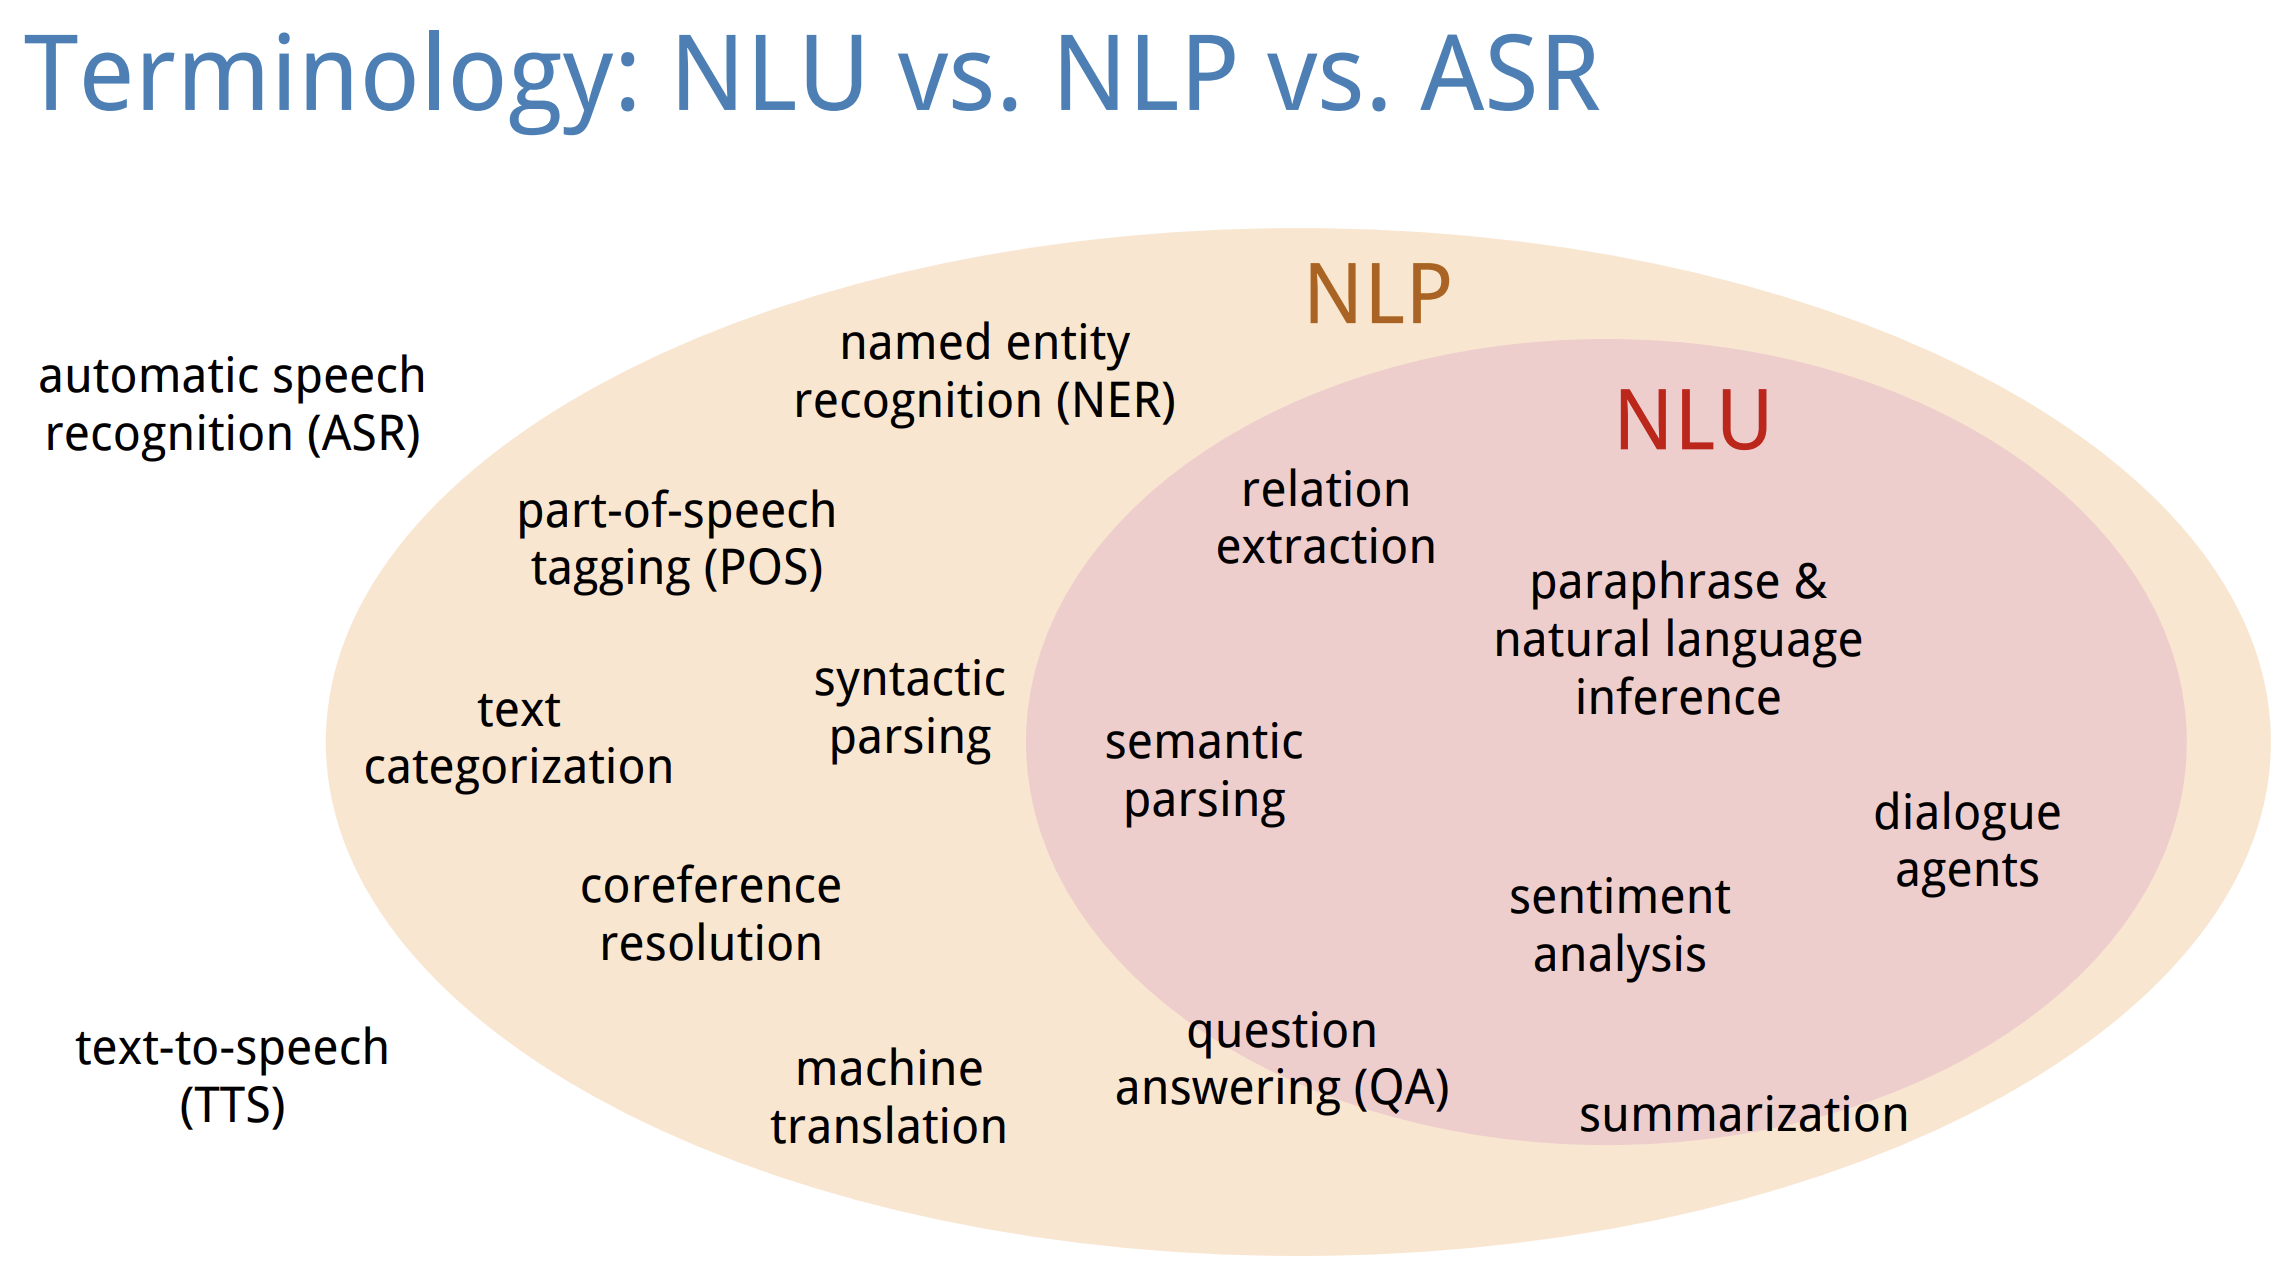
\includegraphics[scale=0.3]{img/f1.png}
\caption{Terminologies their relations}
\label{Fig1: term}
\end{figure}

In the second section, I discussed three core papers in turn. I first discussed the paper "\textbf{Text as Data}" because \cite{10.1257/jel.20181020} introduced why we used text as inputs to economic and social science and how to represent text in a suitable format for scientific analysis. Next, I discussed the paper "\textbf{Interpretable sentiment analysis using the attention-based multiple instance classification model}". \cite{chenyu} proposed a word-level attention-based neural network model for sentiment analysis. Finally, I discussed the paper "\textbf{learning the difference that makes a difference with counterfactually-augmented data}". \cite{DBLP:journals/corr/abs-1909-12434} augmented text data with counterfactual examples to improve the versatility of models. This paper \cite{DBLP:journals/corr/abs-1909-12434} can serve as a future direction of \cite{chenyu} on \href{https://www.winespectator.com/}{wine reviews} for sentiment analysis. 


\section{Analysis of Core Papers}
\subsection{The first paper}
This first paper is called "\textbf{Text as Data}" \cite{10.1257/jel.20181020} written by Matthew Gentzkow, Bryan Kelly, and Matt Taddy. This paper has three main sections: 1. represent text as data, 2. statistical methods, and 3. applications. Human beings started recording and saving digital data dating back to 1940. However, most of them were numeric. Starting from 1980 and beyond, as more people could own personal computers and the internet started to take off, a large amount of digital data has been collected, shared, and saved. Such digital data includes news, articles, books, podcasts, reports, videos, and social media. All kinds of data contain text. In the 1970s, the earliest natural language processing was  \href{https://www.google.com/search?q=regular+expression&sca_esv=596374102&ei=YMOaZbTULdyfqtsP6Y-2kAM&ved=0ahUKEwi0hOz9y8uDAxXcj2oFHemHDTIQ4dUDCBA&oq=regular+expression&gs_lp=Egxnd3Mtd2l6LXNlcnAiEnJlZ3VsYXIgZXhwcmVzc2lvbkgAUABYAHAAeAGQAQCYAQCgAQCqAQC4AQzIAQDiAwQYACBB&sclient=gws-wiz-serp}{regular expression} created in \href{https://www.hpc.iastate.edu/guides/unix-introduction#:~:text=What%20is%20UNIX%3F,for%20servers%2C%20desktops%20and%20laptops.}{Unix Operating System}. Starting from the 1980s, as \href{https://plato.stanford.edu/entries/computational-linguistics/#IntGoaMetComLin}{computational linguistics} was developed, researchers started building machines that could understand texts mimicking humans' brains and interact with humans by parsing the syntax and representing semantic. However, for the past 30 years, researchers in computational linguistics have shifted their perspective of nonprobabilistic syntactic semantics to quantitative probabilistic words in a stochastic process. This later perspective is named \textbf{Statistical NLP}, the mainstream focus to date. One of the most influential Statistical NLP books is called \textbf{"Foundations of Statistical Natural Language Processing"} written by \cite{manning99foundations}.

\subsubsection{Represent Text as Data}
In the last paragraph, I discussed plenty of digital texts, and \textbf{Statistical NLP} is the most effective way to deal with them. However, all traditional statistical methods need numeric inputs. Then, a fundamental question is how we convert texts into traditional data formats. The most straightforward way of representing text in data is to count the appearance of unique words of a corpus in each document. However, in practice, many documents form a corpus. As a result, the dimension of all unique words across all documents is extremely high, making the statistical analysis infeasible. Researchers came up with some ways to reduce the dimensions. The first way is to remove "\textbf{Stop Words}" such as "\textit{a, an, the, for, about, it, and}" and so on. The reason for removing \textbf{Stop Words} is that these words are usually grammatically functional in sentences instead of expressing meanings. Since 1988 \cite{stop} published a list of common stop words for over 40 languages. \cite{tfidf} proposed a very widely used approach, \href{https://en.wikipedia.org/wiki/Tf%E2%80%93idf}{TF-IDF}, to highlight important characteristic words in documents while reducing the commonly used words by assigning different weights to each word. The second way is to filter out words assigned weights by \textbf{TF-IDF} lower than a predefined threshold. \cite{Hiemstra2009} described an alternative method of representing text as data, \textbf{N-Gram}, which uses a phrase of length n as the minimal unit instead of one word. Such a method considers term dependencies and orders. For example, a bigram model counts "\textit{What's up}" as one phrase consistent with human meaning. However, a unigram model counts it as "\textit{What's}" and "\textit{up}", which breaks the original meaning. But dimensions of \textbf{N-Gram} model explode as \textbf{N} increases. As a result, researchers usually first try unigram representation and then evaluate if it is worth trying a 2-gram representation.

All the methods above represent texts as counts. However, counting tokens do not represent all the information conveyed in the text because they ignore word context dependency and word order position. So, researchers have been proposing new ways to represent text as data. \cite{DBLP:journals/corr/MikolovSCCD13} proposed \textbf{Word2Vec} method including \textbf{Skip-Gram} and \textbf{Negative Sampling Algorithm} to train vector representations of words based on their contexts across the whole corpus. The most impressive aspect of this method is that vector representations of words with similar meanings are located in a proximity area of the whole vector space. This means a simple vector operation produces a meaningful result. For example, $$vector("Beijing") - vector("China") \approx vector("Tokyo") - vector("Japan")$$ Without informing models what a country is and capital is, \textbf{Word2Vec} can group words of countries and learn the implicit relations between countries and capitals. Such implicit learning happens to other embeddings. \cite{DBLP:journals/corr/MikolovSCCD13} illustrated their results by the following graph \ref{Fig2: city}, and they built a tool for computing continuous distributed representations of words at \href{https://code.google.com/archive/p/word2vec/}{Word2Vec}.
\begin{figure}[ht]
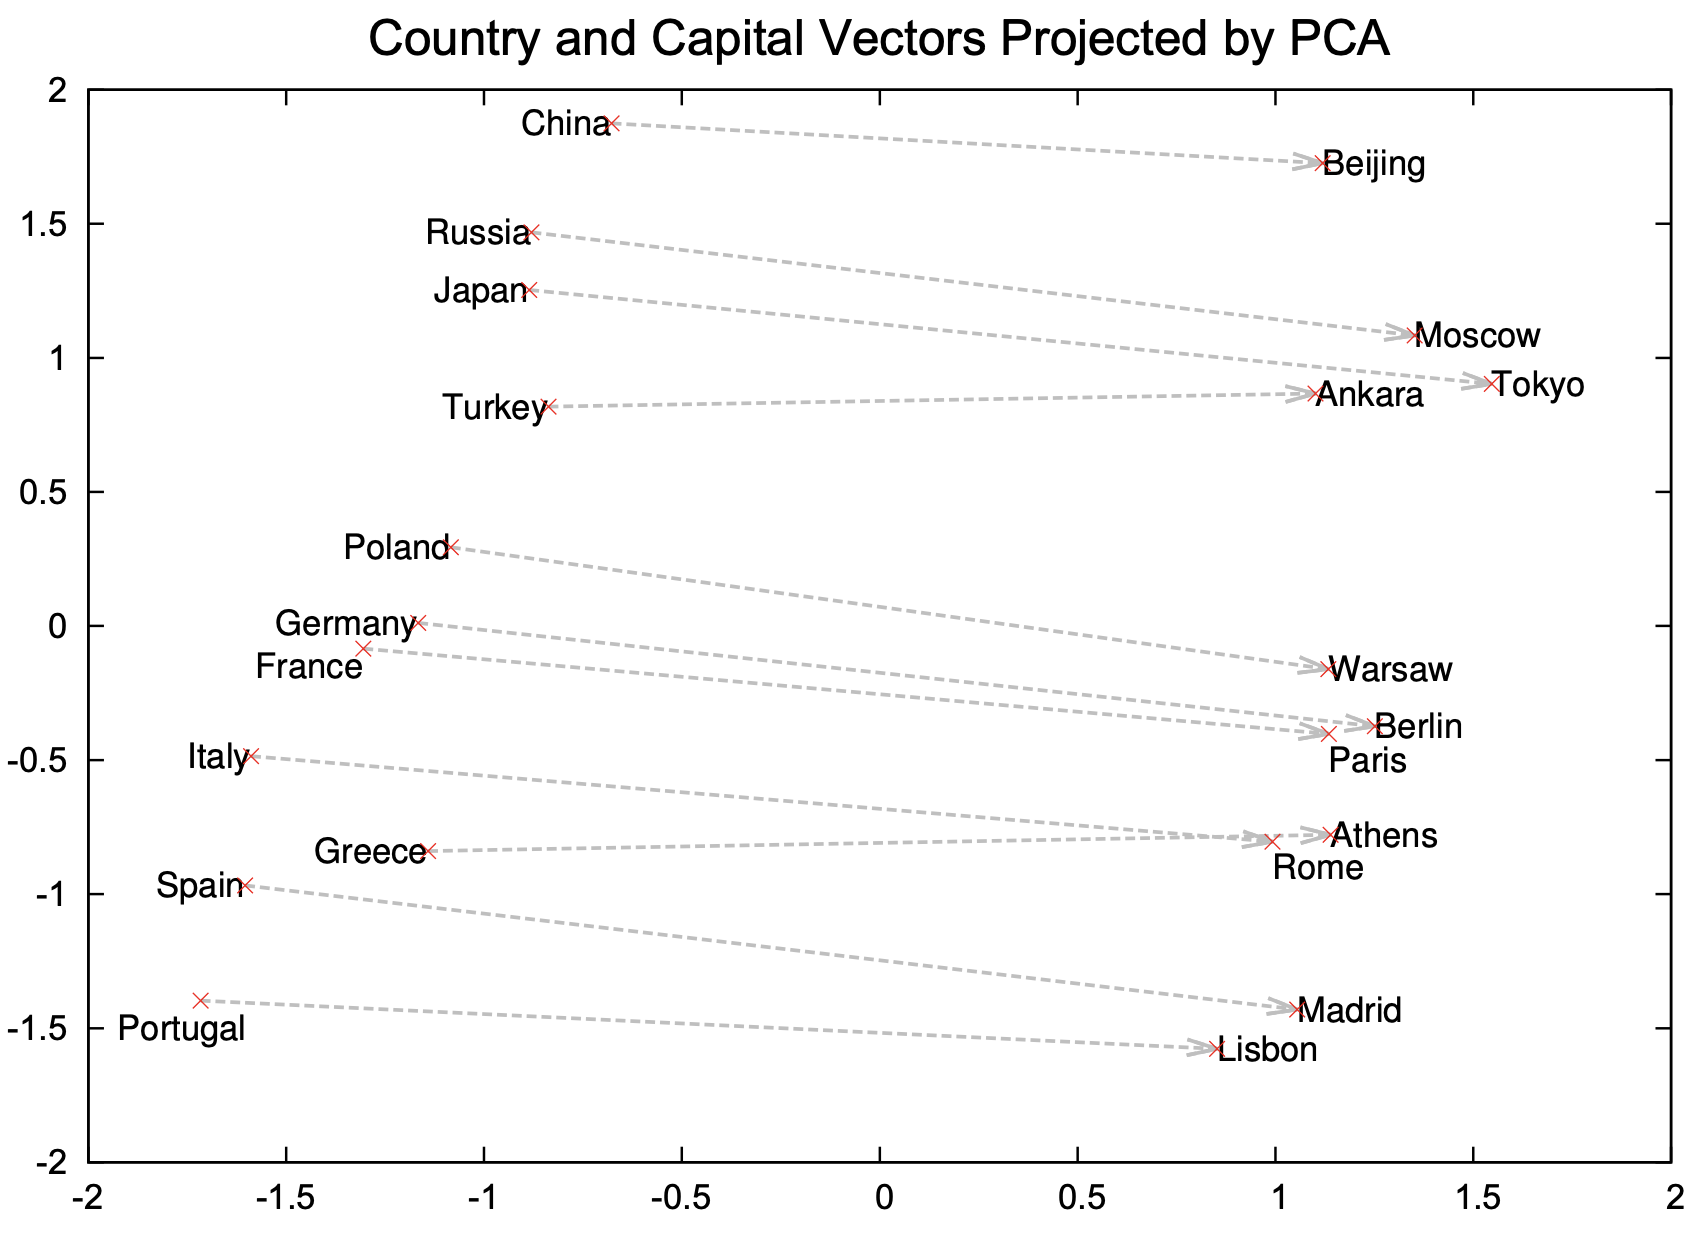
\includegraphics[scale=0.4]{img/city.png}
\caption{Word to Vector Embedding}
\label{Fig2: city}
\end{figure}

Based on the work by \cite{DBLP:journals/corr/MikolovSCCD13}, \cite{pennington-etal-2014-glove} proposed a new method of representing words as embeddings, \textbf{GloVe} (Global Vector). This new method used a word-word co-occurrence matrix to capture global and local contexts. This word-word co-occurrence matrix measures how frequently one word appears near another word across the whole corpus. \cite{pennington-etal-2014-glove} illustrated the conditional probability of a word-word co-occurrence matrix with the following figure \ref{Fig3: co}. The equation "$\frac{P(k|ice)}{P(k|steam)} = 8.9$" from this figure \ref{Fig3: co} indicates that \textit{solid} co-occurs more frequently with \textit{ice} than \textit{steam}. This example is consistent with human logic. As a result, this new method outperformed the \textbf{Word2Vec} method on word analogy tasks and maintained the linear relation property of word embeddings in the vector space. \cite{pennington-etal-2014-glove} built a website and published their project codes for \href{https://nlp.stanford.edu/projects/glove/}{GloVec}.
\begin{figure}[ht]
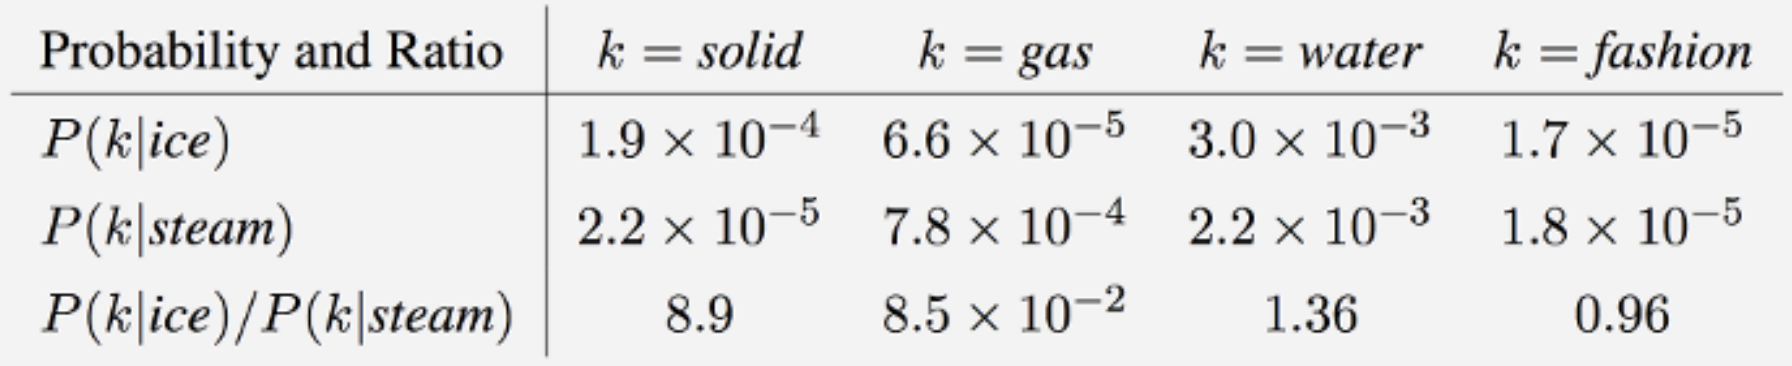
\includegraphics[scale=0.4]{img/co.png}
\caption{Conditional Probability of a Word-Word Co-occurrence Matrix}
\label{Fig3: co}
\end{figure}

\subsubsection{Analysis Methods}
I discussed many methods of representing text as data in the last section. Then, once we have text data, researchers propose many methods to analyze them. There are two groups of methods. The first group is to analyze relationships between token counts and attributes of interest with traditional statistical methods. This group provides interpretations and is ready for causal inference. The second group focuses on predicting attributes of interest with word embeddings and neural networks. This latter group usually has a higher prediction accuracy than the first group. However, it lacks some interpretations and is hard to reason about inference.

The first group of methods can be divided into two subgroups. The first subgroup of methods is \textbf{dictionary-based} methods. For instance, in the case of sentiment analysis, this method classifies documents by counting words in a predefined list to indicate positive or negative tones. \cite{dic} provided some practices about dictionary-based methods. The second subgroup of methods is \textbf{text regression}. \textbf{Text regression} methods regress attributes of interest on  \href{https://en.wikipedia.org/wiki/Document-term_matrix}{document-term count matrix} with traditional statistical methods. Attributes of interest can be sentiment or topics. A simple document-term count matrix is illustrated by the table \ref{tab:doc}.
\begin{table}[ht]
    \centering
    \begin{tabular}{|c|c|c|c|c|} \hline 
         &  I&  love&  hate& you\\ \hline 
         Document 1&  1&  0&  1& 1\\ \hline 
         Document 2&  1&  1&  0& 1\\ \hline
    \end{tabular}
    \caption{Document-Term Matrix}
    \label{tab:doc}
\end{table}
Linear regression is sometimes applied to text regression because it is fast, intuitive, interpretative, and has many statistical properties. However, due to the extremely high dimensions and the sparsity of the document-term matrix, the ordinary linear regression performs poorly on text regression. So, \textbf{Penalized Linear Regression} is applied. \cite{a92f3c16-7c6e-31d3-b403-82d2b0a469e4} introduced biases into estimations of coefficients in multivariate linear regression to reduce the variance and improve model stability. This technique successfully resolves multicollinearity issues. Later \cite{51791361-8fe2-38d5-959f-ae8d048b490d} proposed a new interpretable method, \textbf{Lasso}, that can select variables and make models stable like the ridge regression by a condition that the sum of absolute coefficients needs to be less than a preset constant. This is a cornerstone in the field of statistical methods because \textbf{Lasso} can also be extended to generalized regression models and tree-based models. Combining the ridge regression and lasso, \cite{b61d584f-9c9c-3cf8-b866-214ec2216250} proposed a new regularization and variable selection method named \textbf{Elastic Net} that often outperforms lasso, especially when the number of variables is larger than the number of observations. This applies to the document-term matrix, in which the number of unique tokens (columns) is usually larger than the number of documents (rows). Later, \cite{log} proposed the \textbf{log penalty}, which can be used as a new regularization method. \cite{10.1257/jel.20181020} drew a picture \ref{Fig4: reg} to compare these four regularization functions side by side. Elastic Net is the most widely used penalized term in linear regression.
\begin{figure}[ht]
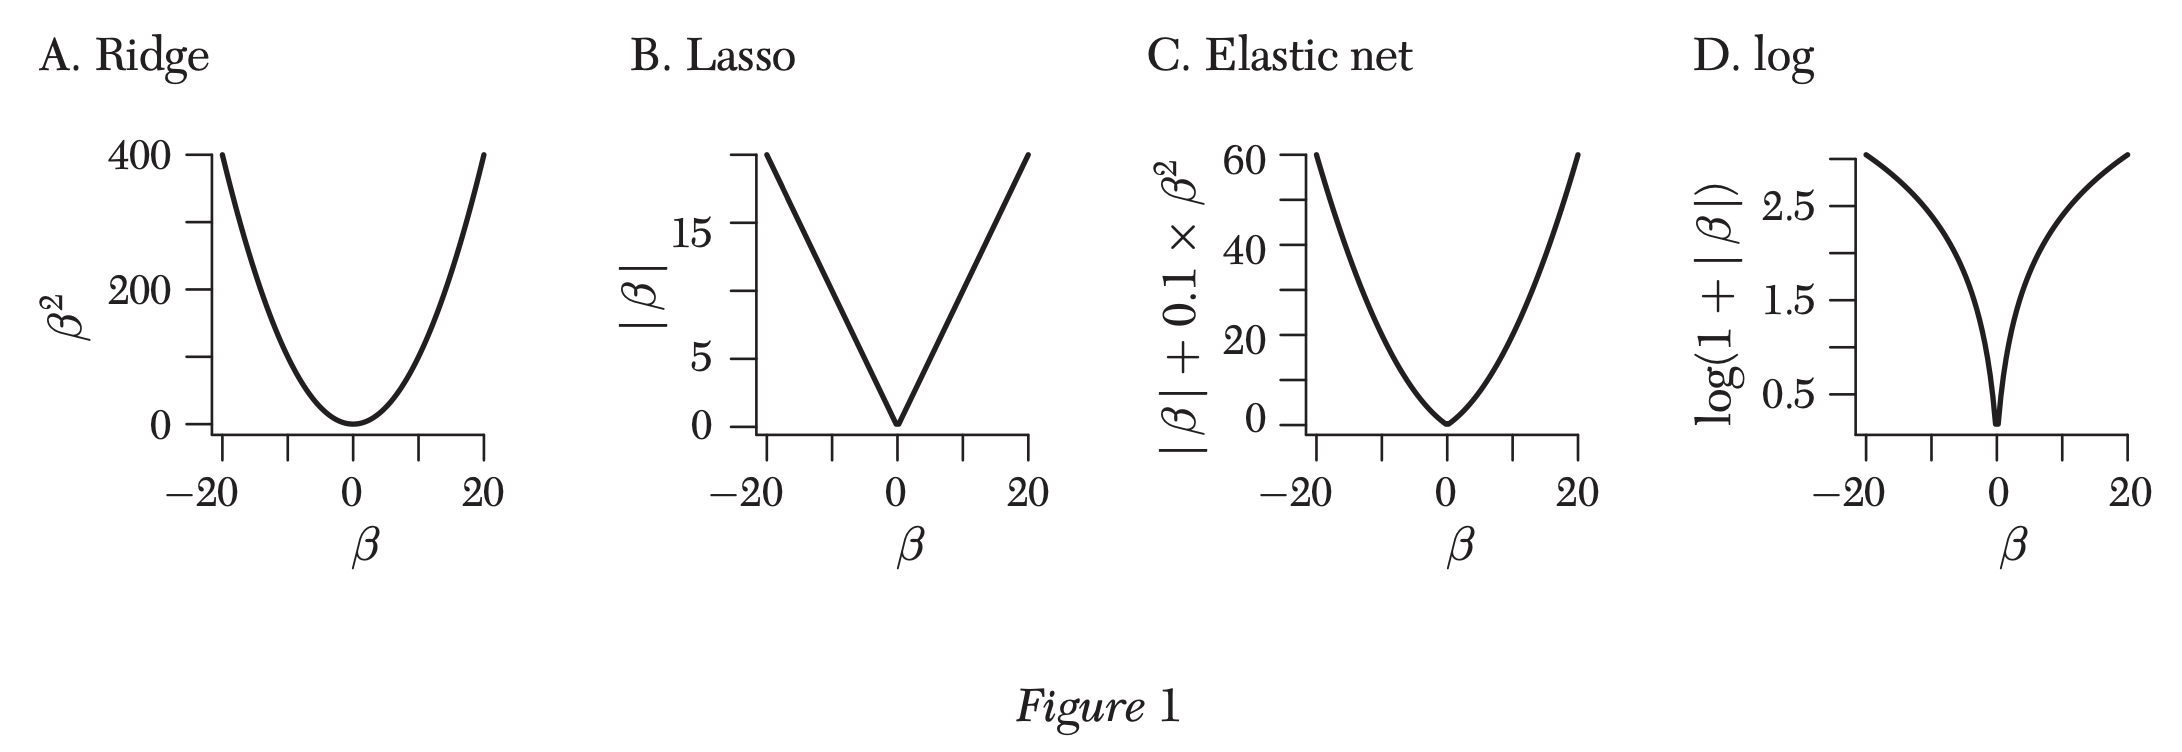
\includegraphics[scale=0.4]{img/reg.png}
\caption{Different regularization functions}
\label{Fig4: reg}
\end{figure}
Another common technique of reducing high dimensions is \textbf{principal component analysis} (PCA) proposed by \cite{1570572700669207808}, which reduces the number of predictors as many as we want while keeping as much information as the original data has. This technique soon became the most popular dimension reduction method in statistics and data science. However, PCA does not consider how the information about attributes affects the structure of all predictors. So, a Swedish statistician \cite{pls} proposed \textbf{Partial Least Regression} to reduce the dimensions by taking advantage of relations between response variables and covariates. \cite{doi:10.1080/01621459.2012.734168} proposed \textbf{Multinomial Inverse Regression} method that reduces the high-dimensional document-term matrix to have a rich information representation in sentiment analysis. He also proposed the \textbf{gamma-lasso} algorithm to get a stable and effective estimation of his new method. The advantage of his method is that it can give an interpretable word loading, which quantifies the degree of sentiment at the word level, and his method is faster to run on a large corpus with limited resources than deep-learning-based methods that I discussed later. \cite{chenyu} compared \cite{doi:10.1080/01621459.2012.734168}'s method with his new method in the second paper. 

All the above-mentioned methods are linear. Although linear models are simple and easy to interpret, many data-generating processes don't follow linearity. Nonlinear text regression is the tool to tackle them. There are three major nonlinear methods used in text analysis – \textbf{generalized linear models}, \textbf{support vector machines}, and \textbf{tree-based models}. \cite{68aee965-a8a0-3e72-9f89-8d89ae91a62b} unified a wide range of statistical models with a common framework, \textbf{generalized linear models}, and provided a unified procedure to fit normal and non-normal data. Their work is a groundbreaking foundation for the whole statistical field. \cite{boser1992training} proposed \textbf{Support Vector Machine} (SVM), which can transform text representations into a higher dimension space where a hyperplane that can divide different classes of texts exists. \cite{rf} proposed a new tree-based method called \textbf{Random Forest}, which can be used for classification and regression tasks. Later, based on random forest, \cite{DBLP:journals/corr/ChenG16} proposed new algorithms that enable \textbf{XGBoost} to compute large-scale data tasks with limited resources. We mostly consider Support Vector Machine, Random Forest, and XGBoost as three major \href{https://en.wikipedia.org/wiki/Machine_learning}{Machine Learning} algorithms. They are applied not only in text analysis but also in other fields by data scientists and statisticians every day. 

Next, I discuss the second group of methods based on neural networks. \cite{bengio2000neural} first applied neural networks to learn distributed representations of words and made language models a significant step into deep learning-based methods. A theoretical foundation supports why deep-learning-based methods work the best among language models. \cite{appro} proposed and proved that a neural network can uniformly approximate any continuous function. This significant desired property is named \textbf{Universal Approximator}. \cite{DBLP:journals/corr/Kim14f} built \textbf{convolutional neural networks} (CNN) to a sentence-level classification task with pre-trained 300-dimension word embeddings from \textbf{Word2Vec} method as inputs proposed by \cite{DBLP:journals/corr/MikolovSCCD13}. His CNN models performed very well on some benchmark datasets, and he remarked on the effectiveness of CNN models in sentiment analysis and question classification. \cite{DBLP:journals/corr/Kim14f} described his simple CNN architecture in the following figure \ref{Fig5: cnn}.
\begin{figure}[ht]
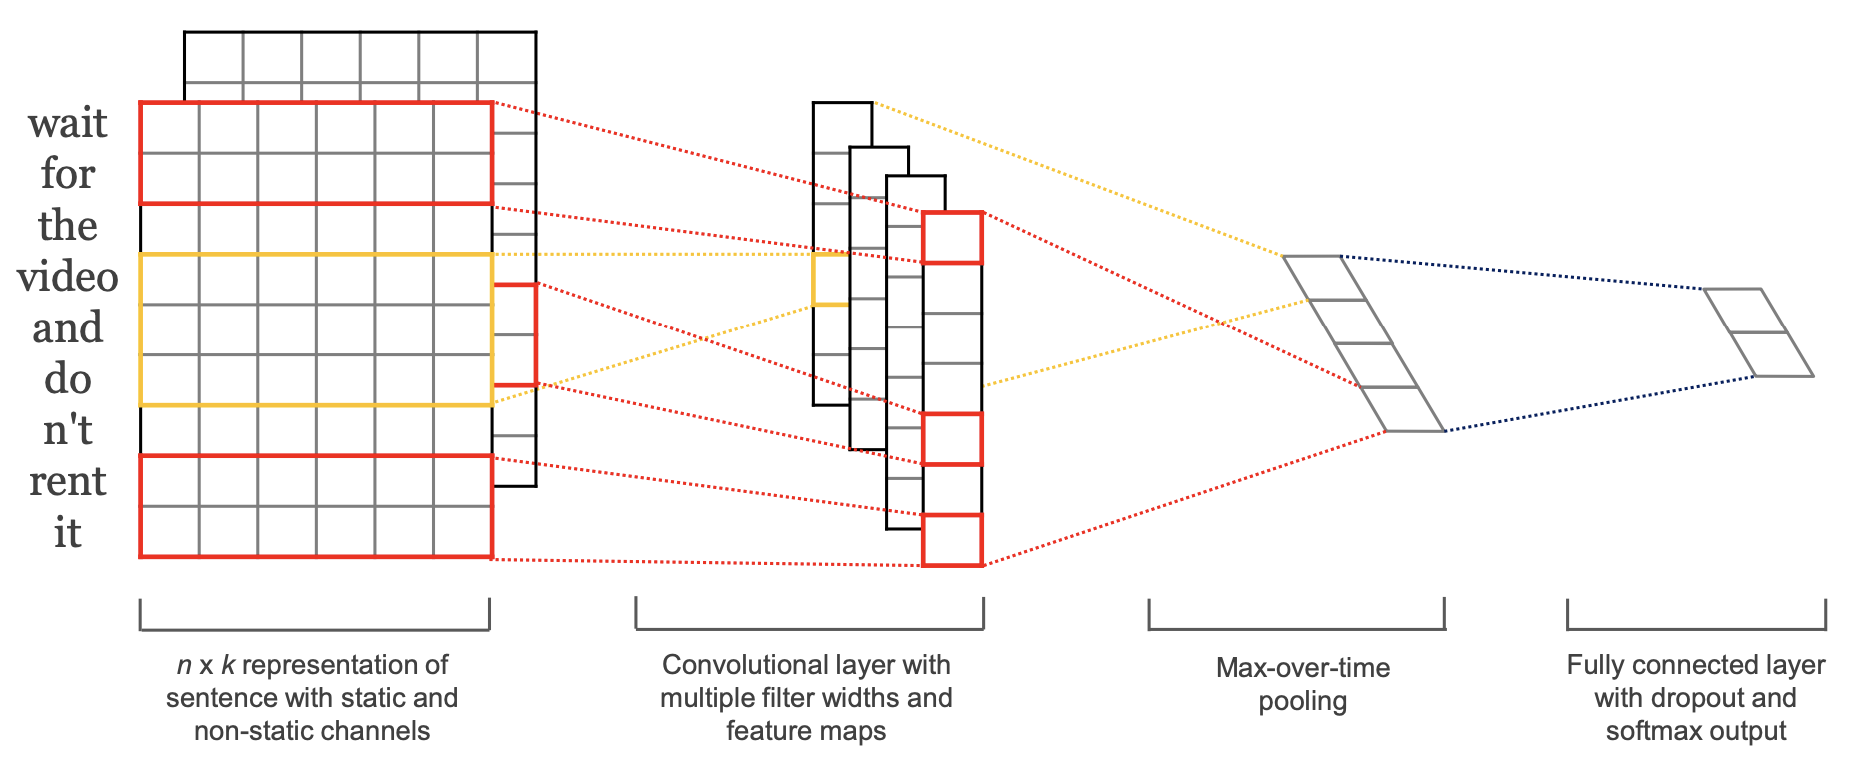
\includegraphics[scale=0.4]{img/cnn.png}
\caption{A simple two-channel CNN architecture in NLP}
\label{Fig5: cnn}
\end{figure}
\cite{10.1162/neco.1997.9.8.1735} proposed a gradient-based method, \textbf{Long Short-Time Memory} (LSTM), that learns to bridge long-time lag tasks. Later, \cite{DBLP:journals/corr/LiuSLW16} applied a word-level bidirectional LSTM (biLSTM) to the Stanford Natural Language Inference Corpus and showed it performed well. Next, \cite{DBLP:journals/corr/VaswaniSPUJGKP17} published a paper called \textbf{Attention Is All You Need}, which revolutionizes the whole field of natural language understanding. It is the foundation of modern language modeling, \textbf{Transformer-based} architecture. The biggest advantage of it is that it captures all words in one sentence at once and pays attention to keywords with the multi-head self-attention mechanism. Previous language models process texts word by word sequentially. As a result, transformer-based models can capture longer dependency contexts. Moreover, it can be easily extended to other language tasks and performs well. \cite{DBLP:journals/corr/VaswaniSPUJGKP17} explained transformer model architecture by the following diagram \ref{Fig5: trans}.
\begin{figure}[ht]
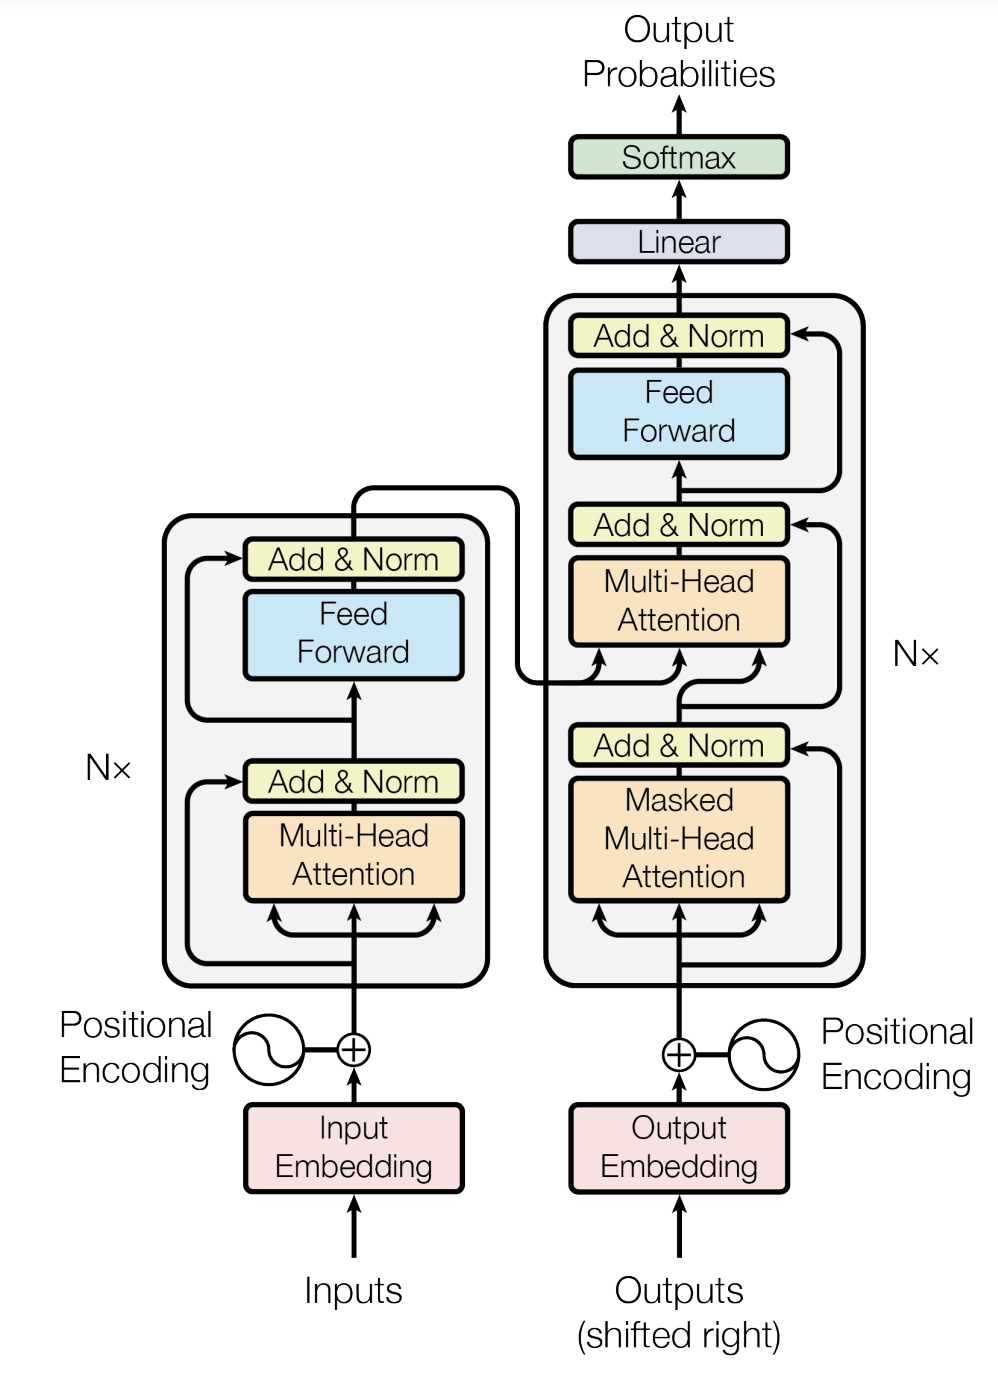
\includegraphics[scale=0.4]{img/trans.png}
\caption{The Transformer Model Architexture}
\label{Fig5: trans}
\end{figure}
Combing \cite{DBLP:journals/corr/LiuSLW16}'s bidirectional LSTM and \cite{DBLP:journals/corr/VaswaniSPUJGKP17}'s transformer model, \cite{DBLP:journals/corr/abs-1810-04805} proposed a new language representation called \textbf{"Bidirectional Encoder Representations from Transformers"}, BERT, which achieved the state-of-art performance on some common dataset. People can add one task-specified layer on top of a pre-trained BERT model. Then, people can fine-tune it for a needed task. Large Language Models are based on BERT, including ChatGPT. 

\subsubsection{Applications} 
Text Analysis can be applied to a wide range of fields. Researchers need it to infer the authorship of debuted articles, books, or text. Economists use it to predict stock prices with news articles. They also use it to measure economic policy uncertainty and its effects. Social scientists use it to observe and interpret news outlets' slants and how they affect or manipulate public opinion. Text analysis is also widely used in law and politics. For instance, integrating congress speeches with time series sheds light on how politics or ideology in a country change as time goes by. 

\subsection{The second paper}
The natural language understanding task in the second paper is sentiment analysis. \cite{DBLP:journals/corr/abs-1801-07883} provided a comprehensive survey of deep learning methods in sentiment analysis. Most deep-learning-based methods are challenging to interpret and make further inferences. Although they achieve state-of-the-art performance in natural language understanding, they are criticized as \textbf{Black Box} to humans. People know they work very well, but people don't know why they work so well. A Ph.D. \cite{Murdoch2019-uy} advised by one of the most Distinguished Statistical Professor \href{https://binyu.stat.berkeley.edu/}{Bin Yu} from UC Berkeley wrote his Ph.D. thesis about interpreting deep learning for natural language processing. \cite{chenyu} proposed a word-level attention-based multiple instance classification model (AMIC). The most significant advantage of the AMIC method is that it provides a word-level context-based sentiment score. This makes a neural network-based model accessible and interpretable. Regarding sentiment analysis, some other researchers have made some progress in interpreting neural networks. 

Next, I dived deeper into the AMIC methodology proposed by \cite{chenyu}. His method aims to do sentiment analysis. There are three main components in AMIC. The first component represents texts as word embeddings with \textbf{GloVec-300-Wiki} proposed by \cite{pennington-etal-2014-glove}. The second component is the Bayesian multiple-instance classification (MIC), proposed by \cite{Xiong2021-zt}. MIC consists of two regression models. The first model is selecting words that express sentiment in one document. The second model uses selected words to make sentiment predictions for one document. The third component uses a self-attention mechanism to capture local and global contexts. It helps the second component select words based on word meaning and contexts.

The second component, MIC, is a core part of the model. \cite{chenyu} drew a figure \ref{Fig6: amic} to show his model architecture. The index $i$ in figure \ref{Fig6: amic} represents the $i^{th}$ document in a corpus. The index $j$ in figure \ref{Fig6: amic} represents the $j^{th}$ word. Then $x_{ij}$ denotes $j^{th}$ word context-independent embedding in $i^{th}$ document. $y_i$ denotes the true $i^{th}$ document sentiment label. Both $x_{ij}$ and $y_i$ are observed. Table \ref{tab:data} illustrates this data structure. MIC consists of two regression models, which can be represented in two layers. 
\begin{table}[ht]
    \centering
    \begin{tabular}{|c|c|c|c|c|} \hline 
         Document ID&  1&  ...&  m& label\\ \hline 
         1&  $x_{11}$&  ...&  $x_{1m}$& positive\\ \hline 
         ...&  ...&  ...&  ...& ...\\ \hline 
         n&  $x_{n1}$&  ...&  $x_{nm}$ & negative\\ \hline
    \end{tabular}
    \caption{Data Structure}
    \label{tab:data}
\end{table}

The right blue dashed square box in figure \ref{Fig6: amic} represents layer one, which is trained to get indicator values, $\delta_{ij}$. $\delta_{ij}$ represents the degree of how much $j^{th}$ a word in a $i^{th}$ document expresses in sentiment. Three computing processes exist before getting $\delta_{ij}$. The first process trains the context-independent word embeddings $x_{ij}$ into context-dependent word embeddings $a_{ij}^P$ with a self-attention mechanism. The second process fits a logistic regression that takes $a_{ij}^P$ as input and returns $u_{ij}$ as output, the logistic-regression probabilistic score. $b$ is the logistic regression coefficient. The third process converts $u_{ij}$ into $\delta_{ij}$ with a  \href{https://en.wikipedia.org/wiki/Sigmoid_function#:~:text=A%20sigmoid%20function%20is%20a,refer%20to%20the%20same%20object.}{sigmoid function} as follows: $$\delta_{ij}=\frac{1}{1+e^{-u_{ij}}}$$ The reason for using a sigmoid function is that the backpropagation training needs a differentiable function. \cite{chenyu} also applied two penalty terms, $p_{i1}$ and $p_{i2}$, to the final $\delta_{ij}$. The penalty term one $p_{i1} = c_1\sum_{j=1}^m(\delta_{ij}(1-\delta_{ij}))^{1/2}$ pushes all values of $\delta_{ij}$ to be close to either 1 or 0 boundaries. $c_1$ is a hyperparameter that can be tuned. The penalty term two $p_{i2} = c_2\sum_{j=1}^m\delta_{ij}$ controls the density of sentiment words in one document. There are fewer sentiment words if the tuning parameter $c_2$ is large, and vice versa. The second penalty term is because every document only has a few sentiment words. If all words are used to predict the final document sentiment, lots of noise decreases the prediction performance. 

The left red dashed square box in figure \ref{Fig6: amic} represents layer two. The goal of layer two trains the final document sentiment prediction $Z_{i}$ to match the true sentiment label $y_i$ with the selected words by layer one. The second layer has four processes. The first process trains context-independent word embeddings $x_{ij}$ into context-dependent word embeddings $a_{ij}^L$. Although this first process in layer two has the same procedure as the first process in layer one, the self-attention training weights are different. This is because the two self-attention transformations have different purposes. The second process fits a logistic regression that takes $a_{ij}^L$ as inputs and returns $Z_{ij}$ as outputs. $Z_{ij}$ is the sentiment score of the $j^{th}$ word in the $i^{th}$ document. $\beta$ is the logistic regression coefficient. The third process averages all $Z_{ij}$ at the word level in the $i^{th}$ document to get the document-level sentiment score $Z_{i}$. The fourth process applies two activation functions to $Z_{i}$. The first function is the same sigmoid function used in the first layer. The second function is the indicator, which uses 0.5 as the threshold. If the $S(Z_i)$ is larger than 0.5, the final prediction is 1; otherwise, it is zero. \cite{chenyu} also applied a third penalty term $p_{i3}=c_3\sqrt{\sum_{j=1}^m(a_{ij^L\beta})^2}$ to control the absolute magnitude of $Z_{ij}$. This ensures that $Z_{ij}$ is stable during training.
\begin{figure}[ht]
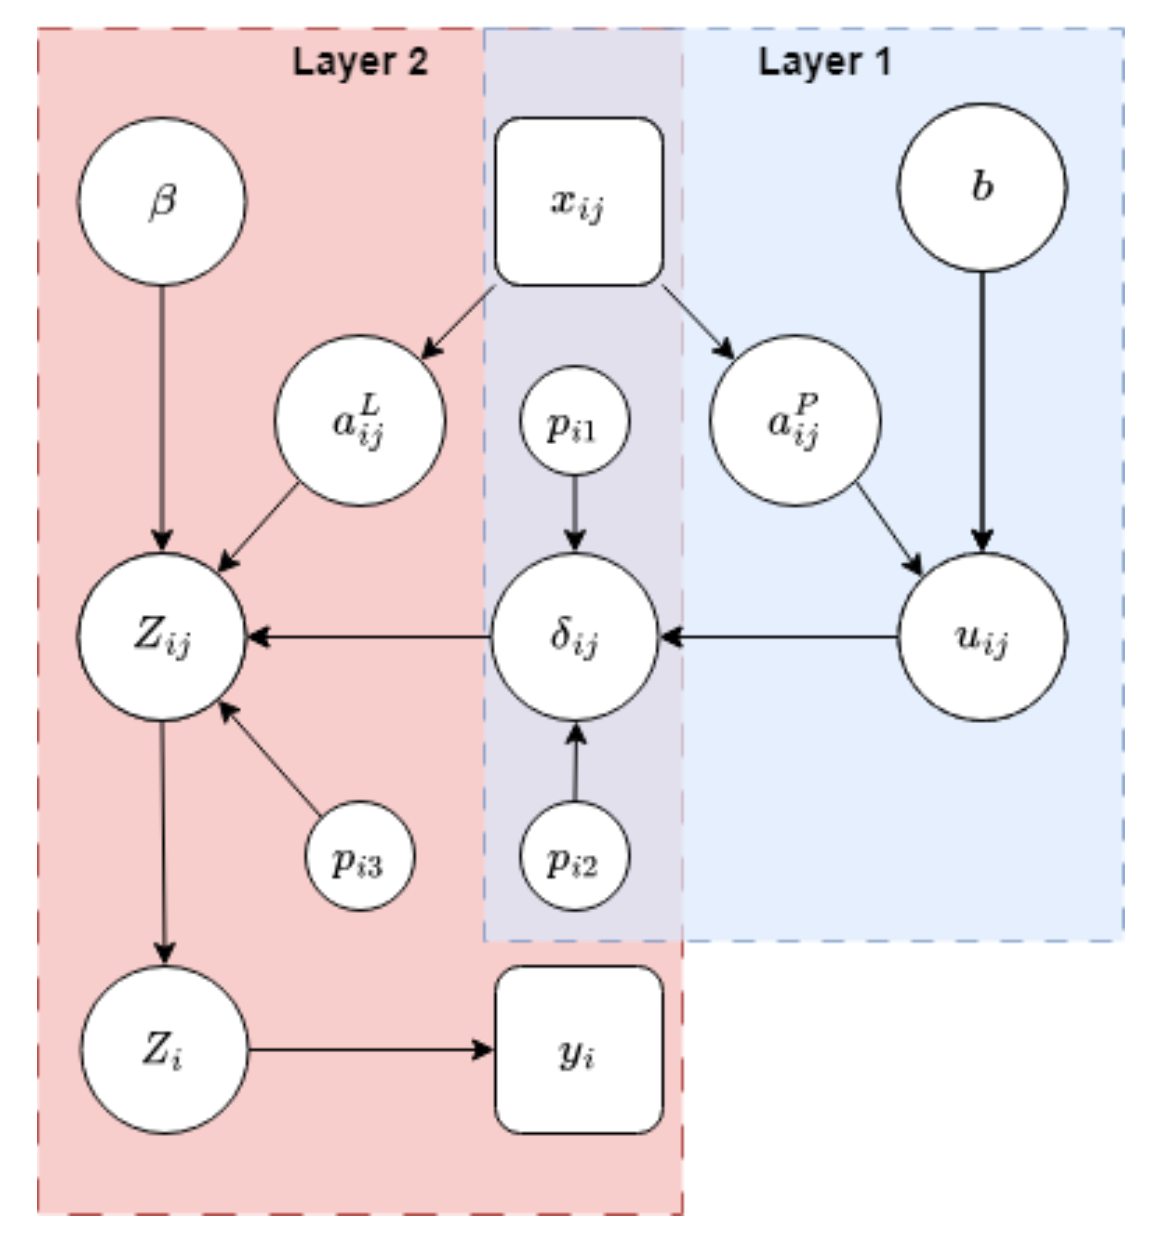
\includegraphics[scale=0.4]{img/amic.png}
\caption{The Anatomy of AMIC Model}
\label{Fig6: amic}
\end{figure}

The last part of this model is the final objective function, as follows $$Obj(x_{ij}, y_i)=-\frac{1}{n}\sum_{i=1}^n\left[\left(y_i\log(S(Z_i))+(1-y_i)\log(1-S(Z_i))\right)+p_{i1}+p_{i2}+p_{i3}\right]$$ Because sentiment analysis is a classification task, the \href{https://en.wikipedia.org/wiki/Cross-entropy}{cross-entropy loss} is applied in the above objective function. This training process is neural-network-based, so stochastic gradient descent with backpropagation minimizes the objective function. 

\cite{chenyu} applied his novel AMIC method to a wine review dataset proposed by \cite{katumullage_yang_barth_cao_2022} and \cite{yang_barth_katumullage_cao_2022} to evaluate its performance. This wine review dataset has 141,409 reviews. A numeric variable in this dataset called \textit{rating} ranges from 80 to 100. \cite{chenyu} dichotomized this \textit{rating} variable by labeling numbers less than 90 as negative, otherwise positive. After transforming the response variable, \cite{chenyu} preprocessed input reviews. He made all reviews have the same length, 150. He also removed words in reviews that didn't exist in \textbf{GloVe-300-Wiki} vocabulary. He removed punctuations, and he converted all words to lowercase. He didn't remove stop words and didn't stem all words. 

\cite{chenyu} implemented his AMIC with \href{https://pytorch.org/}{PyTorch} in Python. He split this wine review dataset into training, validation, and testing by a ratio of 18:1:1. The final AMIC model prediction accuracy is reported on the testing set with the parameters that produced the lowest loss on the validation set. The following table \ref{tab:acc} compares AMIC with other document-level state-of-the-art neural-network-based models – CNN, BERT, and BILSTM. This table \ref{tab:acc} is sorted descending by accuracy. \cite{chenyu} also compared AMIC with another statistical word-level model, MNIR proposed by \cite{doi:10.1080/01621459.2012.734168}. MNIR was run in R with \href{https://cran.r-project.org/web/packages/textir/index.html}{textir} and \href{https://cran.r-project.org/web/packages/tm/vignettes/tm.pdf}{tm} packages. It took a normal CPU computer a few minutes to finish. All other neural-network-based models were run in \href{https://colab.research.google.com/}{Google Colab}. It took a normal GPU on \textit{Google Colab} between 20 and 30 minutes to finish the AMIC, CNN and BILSTM models. It took a normal GPU about 2 hours to finish the BERT model. AMIC achieved the highest test accuracy, 89.26\%. BERT, BILSTM, and CNN also achieved around test accuracy of 88\%, which is very close to the AMIC. MNIR achieved a bit lower test accuracy, 84.68\%. However, MNIR took much less time and much fewer resources than neural-network-based models to achieve a word-level interpretable model with only a bit lower accuracy. This arouses us to ask if it is worth applying neural-network-based models to a simple sentiment classification task. 

The advantage of AMIC is that it combines statistical interpretability with deep-learning-based high predictive ability. It can identify sentiment words, especially used in wine reviews, that are not used to express sentiment in daily language usage. A self-attention mechanism achieves this context-based word embeddings. The drawback of \cite{chenyu}'s paper is he only evaluated this novel method on a selected wine review. To show the generality of a novel method, authors need to either simulate many different kinds of data or evaluate a method on a wide range of existing datasets. Another drawback of AMIC is that it doesn't consider the positions of words.

\begin{table}[ht]
    \centering
    \begin{tabular}{|c|c|} \hline 
           Model& Predictive Accuracy\\ \hline 
           AMIC& 89.26\%\\ \hline 
           BERT& 89.12\%\\ \hline 
           BILSTM& 88.69\%\\ \hline 
           CNN& 88.02\%\\ \hline 
           MNIR& 84.68\%\\ \hline 
           MNIR (bigram)& 83.45\%\\ \hline
    \end{tabular}
    \caption{Model Predictive Accuracy}
    \label{tab:acc}
\end{table}

\subsection{The third paper} In this section, I discussed the third paper, "Learning the difference that makes a difference", written by \cite{DBLP:journals/corr/abs-1909-12434}. The main point of this paper is that some researchers found that neural network-based models only use surface-level patterns or associations of data to finish the task. \cite{DBLP:journals/corr/abs-1909-12434} found that this phenomenon greatly affected the generalizability of "sentiment analysis" models and "natural language inference" models. Models that are trained on the original dataset perform poorly on the counterfactual-revised counterparts. One reason for this phenomenon, I assumed, is that neural-network-based models are "black boxes," which makes researchers hardly control what truly works in such complicated models under the hood. Another reason is that neural-network-based models are so easy to overfit that they perform poorly on the out-of-sample data. So, he proposed a method that makes natural language processing models more versatile. The novel method allows humans to create new observations with counterfactual texts and labels according to the original observations. This creation requires that new observations make sense and edits are minimized. \cite{DBLP:journals/corr/abs-1909-12434} elucidated this human-in-the-loop data augmentation by figure \ref{Fig7: aug}. Then, he retrained models on combining the original and newly created datasets. As a result, he found that such models are less sensitive to surface-level patterns. Such models achieved a bit lower accuracy on the original dataset than those trained only on the original one. However, it performs much better on the counterfactual-revised counterparts than those trained only on the original. He revised an IMDB movie review dataset proposed by \cite{maas-etal-2011-learning} for sentiment classification. This IMDB review dataset was split into 1707 training, 245 validation, and 488 tests. He revised the "Stanford Natural Language Inference Corpus" proposed by \cite{bowman-etal-2015-large}, the popular benchmark data for natural language inference tasks (NLI). He randomly sampled 1750 training, 250 validation, and 500 tests from the SNLI. Then, he asked workers to revise the premises and hypothesis, respectively. Lastly, he got 6664 pairs of training, 800 pairs of validation, and 1600 pairs of tests. Sentiment Analysis is usually a binary classification task, positive or negative. NLI is usually a 3-way classification task. NLI classifies a pair of premises and hypotheses into three relations – entailment, contradiction, and neutral.
\begin{figure}[ht]
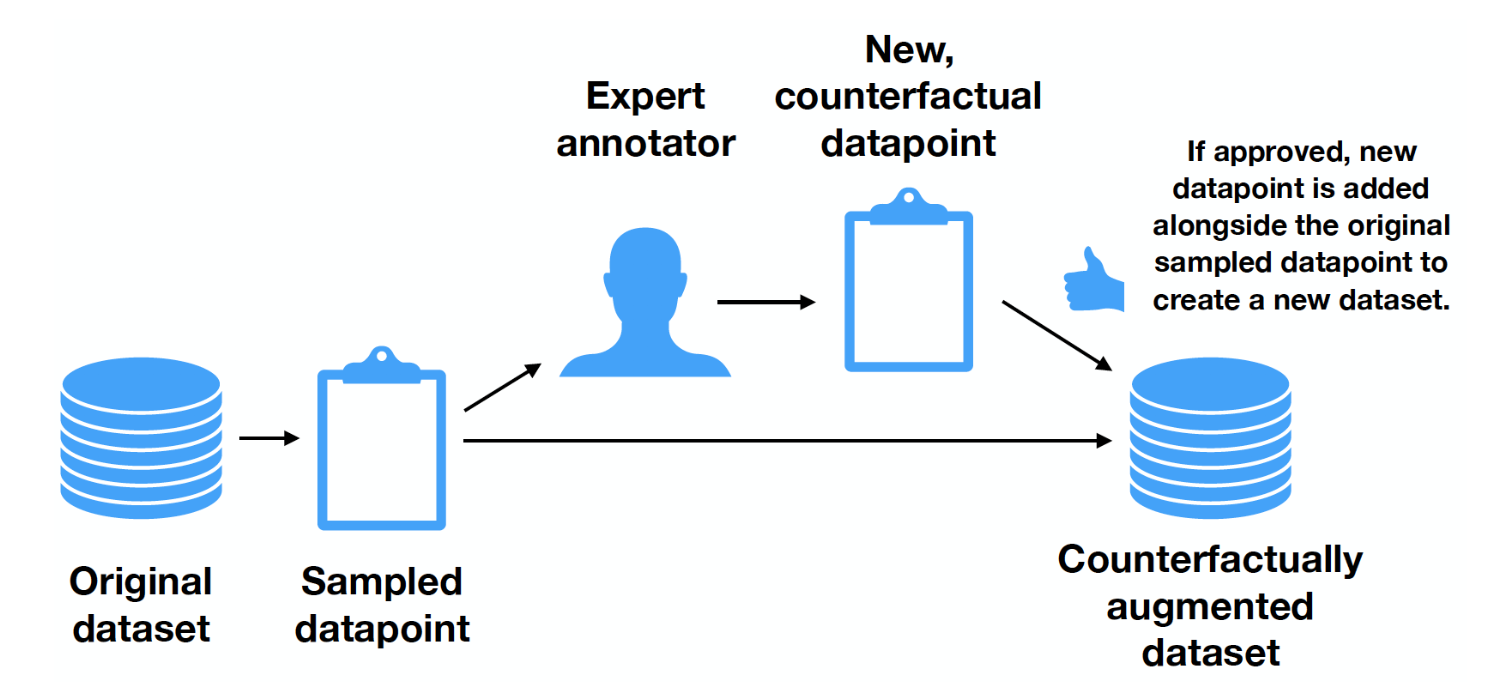
\includegraphics[scale=0.4]{img/aug.png}
\caption{The process of augmenting dataset}
\label{Fig7: aug}
\end{figure}

\cite{DBLP:journals/corr/abs-1909-12434} evaluated his novel method with five models – Support Vector Machine (SVM), Naïve Bayes Model (NB), BILSTM, ELMo-LSTM, and BERT. They used \textit{scikit-learn} package to run the SVM and NB model for sentiment analysis. They used \textit{PyTorch} package to run BILSTM, ELMo-LSTM, and BERT model. After evaluations, they found it worth paying extra to let models learn the surface-level and deep-level patterns by augmenting data with counterfactual instances. They also evaluated their models on out-of-domain datasets, including Amazon reviews, the Twitter sentiment dataset, and Yelp reviews. They showed that models trained on the counterfactual-augmented dataset performed better than those trained only on the original dataset. For example, the BILSTM model trained on the combined dataset (the original and the revised) achieved 82.7\% accuracy on the Amazon review dataset for sentiment analysis. However, the BILSTM model trained only on the original dataset achieved 65.9\% accuracy on the same Amazon review dataset. The full evaluation result tables are displayed in \cite{DBLP:journals/corr/abs-1909-12434}'s paper. The advantage of their novel method is that counterfactual-augmented datasets push models to learn the non-surface-level texture and patterns. For instance, in the IMDB movie review dataset, \textit{"horror"} and \textit{"romantic"} are two movie genre words. However, the SVM models trained only on the original or revised data selected these two movie genre words as sentiment words. This shows models trained on a partial dataset learn something wrong in sentiment analysis. But, when the SVM model was trained on the combined dataset, \textit{"horror"} and \textit{"romantic"} were not selected to be sentiment words. Instead, words such as \textit{"poorly"} and \textit{"awesome"} were selected. \cite{DBLP:journals/corr/abs-1909-12434} elucidated the above phenomenon "Learn the difference what makes a difference" in the figure \ref{Fig8: com}.
\begin{figure}[ht]
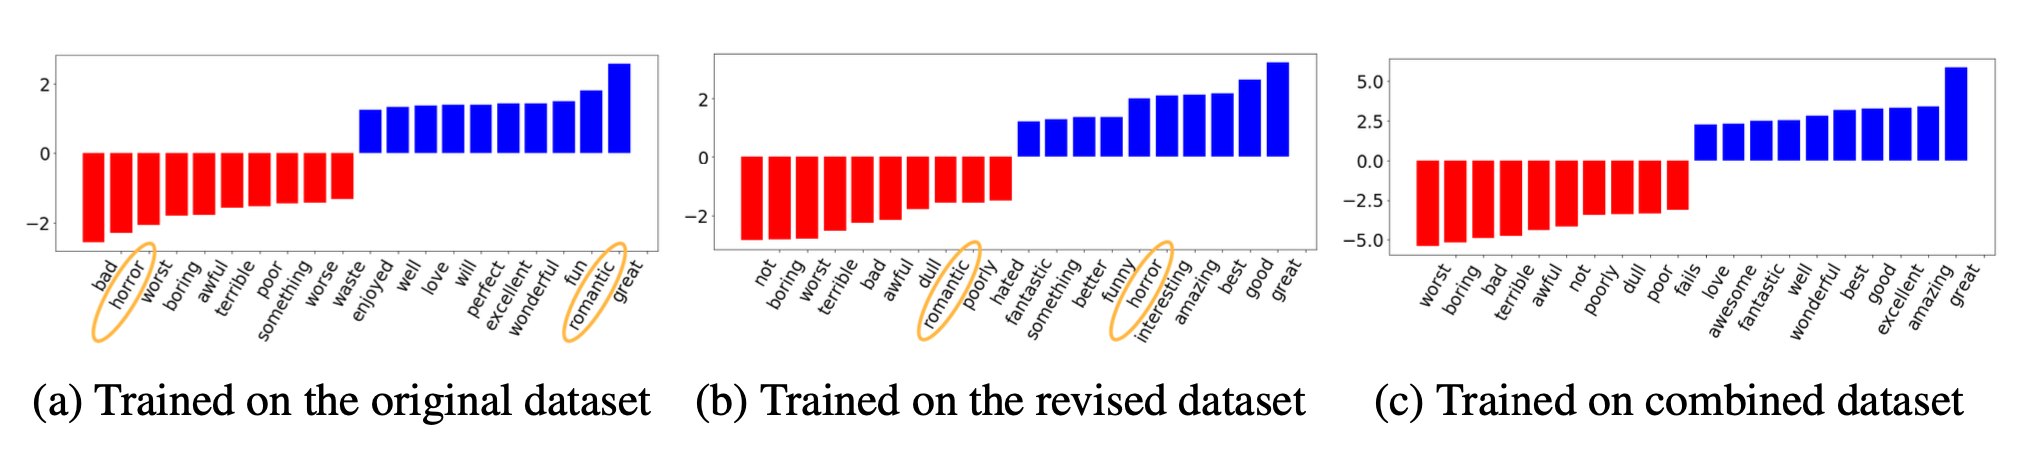
\includegraphics[scale=0.4]{img/com.png}
\caption{Different sentiment words selected by SVM on different kinds of data}
\label{Fig8: com}
\end{figure}

The same "drop" phenomenon happened to the NLI task. For example, the BERT model trained only on the 8,300 original data achieved 77.8\% accuracy on the original data. However, it only achieved 44.6\% accuracy on the revised-premise dataset and 66.1\% accuracy on the revised-hypothesis dataset. However, the BERT model trained on the combined dataset achieved 73.5\% accuracy on the original, 64.6\% accuracy on the revised-premise data, and 69.6\% accuracy on the revised-hypothesis data. 

Overall, counterfactual-augmented data helps models learn the non-surface-level pattern. This makes them versatile and general in sentiment analysis and natural language inference tasks.

\section{Synthesis of Core Papers} After discussing the above three core papers, I summarized and synthesized them in this section. The relation of these papers is a linear sequence. The first paper, "\textbf{Text as Data}" written by \cite{10.1257/jel.20181020}, aims to survey methods of representing text into numeric data. This paper gives us a collection of ways to prepare data. The second paper, "\textbf{Interpretable Sentiment Analysis Using the Attention-Based Multiple Instance Classification Model}" written by \cite{chenyu}, proposed an attention-based multiple instance classification model (AMIC). He used two methods of representing text as data, discussed in the first paper \cite{10.1257/jel.20181020}. The first method counts the n-gram tokens in documents, forming the document-term matrix. He used this document-term matrix to run the baseline sentiment analysis model – MNIR- discussed in the first paper. The second method is \textbf{GloVe-300-Wiki}, which represents words into context-independent embeddings. He applied this method in his novel proposed AMIC. \cite{10.1257/jel.20181020} also discussed many applications in sentiment analysis. \cite{10.1257/jel.20181020} thought in social science and economics, it is useful and important to have model interpretability and causal inference. However, they found most state-of-the-art neural-network-based models don't provide any interpretations, though they can achieve much higher predictive accuracy than traditional statistical methods. \cite{chenyu} positively addressed their issue by proposing AMIC, which can give word-level sentiment scores. This neural network method provides accessibility and interoperability. The third paper, "\textbf{Learning the Difference that makes a difference with Counterfactually-Augmented Data}" written by \cite{DBLP:journals/corr/abs-1909-12434}, pointed out that some NLP models only learn the surface-level patterns of data to make predictions in sentiment analysis and natural language inference. This drawback makes these NLP models perform poorly on the out-of-sample and sensitive to these learned surface-level patterns. However, \cite{chenyu} didn't augment the \textit{wine review} data with counterfactual instances for evaluating his novel AMIC on sentiment analysis. This makes us think about if \cite{chenyu}'s AMIC for sentiment analysis suffers the same issue as \cite{DBLP:journals/corr/abs-1909-12434} pointed out. As a result, the third paper can be used to test if AMIC has the same issue. If so, the third paper is a future direction for augmenting the \textit{wine review} dataset with counterfactual instances. Then, AMIC will be trained on this augmented data to generalize and make it less sensitive to the surface-level patterns. However, augmenting \textit{wine review} data is a big challenge. It requires many human efforts to revise the original data manually to some scale level. This costs a lot of money and time to finish. Whether it is worth augmenting data depends on the application and its purpose. If a wine company wants to monitor their wine product quality by their customers' reviews and further improve their wine, I think for this company, it's worth investing money and resources to augment data. However, for researchers, because of limited resources, creating a few toy counterfactual examples and testing the performance of AMIC on it is enough. 
\begin{figure}[ht]
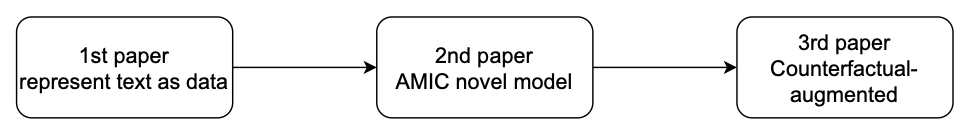
\includegraphics[scale=0.7]{img/re.png}
\caption{The linear sequence of three core papers}
\label{Fig9: re}
\end{figure}

From the results of the second and the third papers, before experiments, I assume counterfactual instances of \textit{wine review} could further improve the generalizability of the AMIC model. However, I think the degree of improvement is limited. I explained my assumption as follows. In Figure \ref{Fig9: re}, I discussed that models trained only on the original dataset \textit{IMDB} selected movie genre words such as \textit{"horror"} and \textit{"romantic"} as highly weighted sentiment indicators. But models trained on the counterfactual-augmented dataset replaced movie genre words with exact sentiment-expressing words such as \textit{"poorly"} and \textit{"awesome"}. In the \cite{chenyu}'s paper, he displayed the AMIC top 50 positive sentiment words in table \ref{Fig10: pos}. I found that words that express the actions of tasting wines, such as \textit{"drips"} and \textit{"soak"}, were picked up by AMIC model as top positive sentiment words. These action words are usually considered neutral in the sentiment analysis. However, most of the top 50 sentiment words in this table \ref{Fig10: pos} expressed positive. Retraining the AMIC model on a counterfactual-augmented \textit{wine review} could help it learn more non-surface-level patterns and generalize well to out-of-domain data, but the degree of improvement is determined by how many counterfactual instances are created and the quality of them.
\begin{figure}[ht]
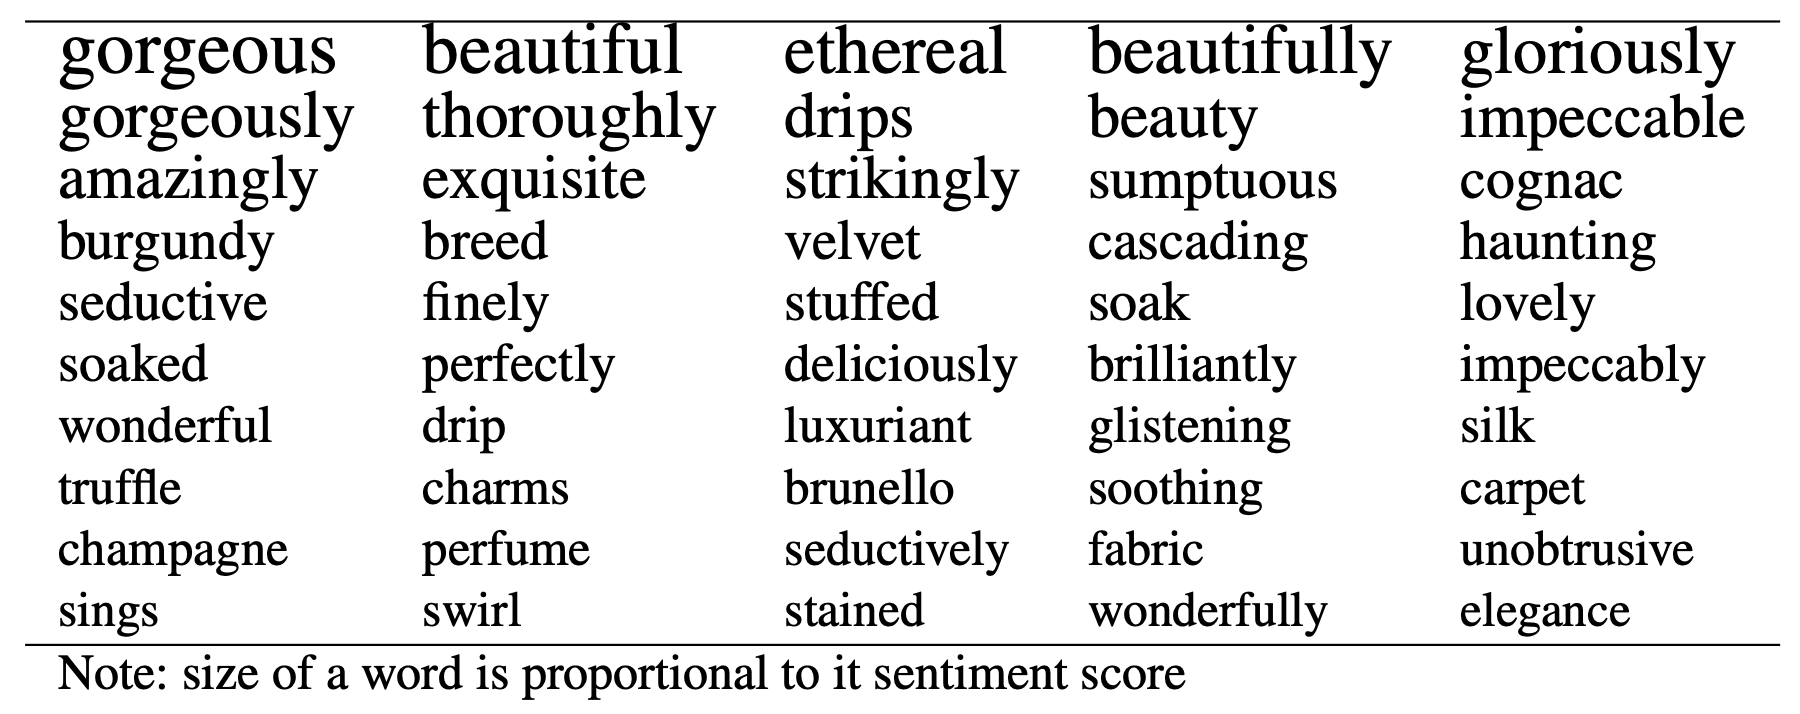
\includegraphics[scale=0.4]{img/pos.png}
\caption{AMIC's top 50 positive sentiment words}
\label{Fig10: pos}
\end{figure}

\section{Technical Details}
After discussing each core paper and synthesizing them, researchers must be able to reproduce and validate the results of novel methods and validate them. \cite{belz-etal-2021-systematic} found that in the natural language understanding area, only a small percentage of papers' results can be reproduced to have the same results under the same conditions shown in the original papers. They also found that the reproduction results were usually worse than reported in the original papers if a discrepancy happened. In natural language understanding, now there is no clear definition of reproducibility and how researchers should measure it. Although there is no clear definition, my measurement is to try to get the test accuracy as close to the report as possible.  

I reproduced the AIMC model performance results for sentiment analysis in this section. The table I reproduced in the second paper, written by \cite{chenyu}, is shown on Page 9. His table is shown in the below figure \ref{Fig11: per}. I reordered each model's predictive accuracy in descending order in table \ref{tab:acc} when I discussed his paper in section two. 
\begin{figure}[ht]
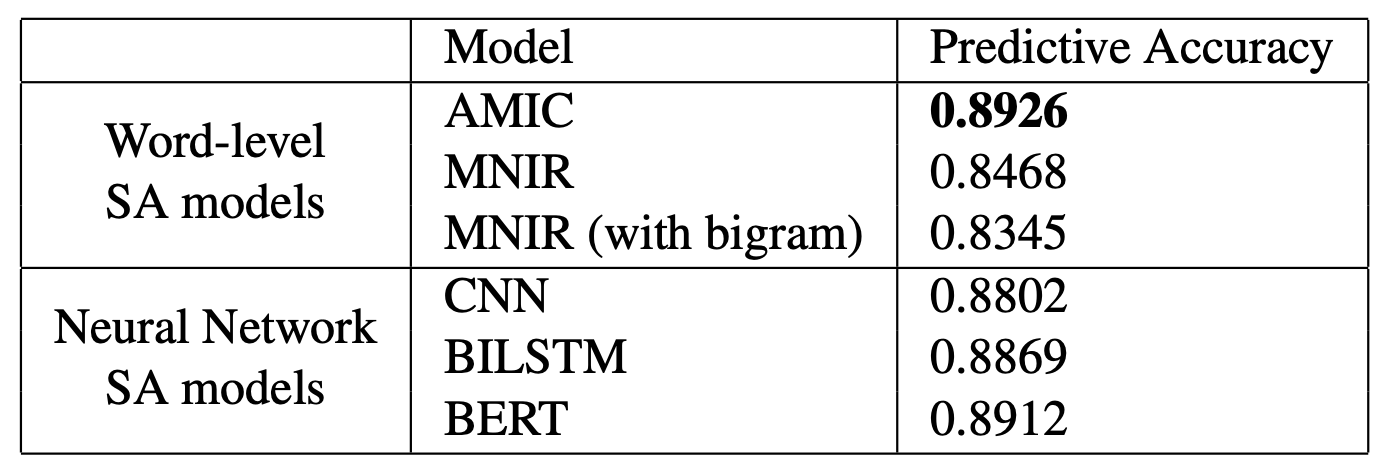
\includegraphics[scale=0.4]{img/per.png}
\caption{Compare AMIC performance with other models}
\label{Fig11: per}
\end{figure}

I explained the whole process of my reproduction of his novel AMIC method and some other models shown in the table \ref{Fig11: per}. Regarding AMIC, luckily, when I contacted the author \href{chenyuy@smu.edu}{Chenyu Yang} about reproducing his results, he shared me with his \href{https://jupyter.org/}{Jupyter Notebooks} that included his codes of building his AMIC and some simple inference of results. He also gave me the dataset used to evaluate AMIC in the second paper. The dataset is \textit{wine reviews}, which has 141,409 observations and was collected from \href{https://www.winespectator.com/}{Wine Spectator} from 2005 to 2016. This dataset was shared in an Excel format. He also shared the \textbf{GloVe} word embeddings of 300 dimensions. All the above files were shared via \href{https://www.smu.edu/OIT/Services/Box}{SMU Box}.

Regarding AMIC, I used the \href{https://colab.google/}{Google Colab} to run his codes. T4 GPU and High-RAM were used to compute. His AMIC was implemented in \href{https://pytorch.org/}{PyTorch}. The torch version is \textit{"2.1.0+cu121"}. The \textit{wine reviews} data was stored in \href{https://www.google.com/drive/}{Google Drive}, and it was read in colab into a pandas format. The dataset has ten variables, but only \textit{rating} and \textit{Clean\_desc} variables were used. He then shuffled the data with a random seed = 42. Then, there are many preprocessing steps to represent review descriptions in data. First, reviews were tokenized by \href{https://www.tensorflow.org/api_docs/python/tf/keras/preprocessing/text/Tokenizer}{Tokenize}, and a dictionary of mapping token IDs to words was created. Second, he initialized a word-embedding dictionary with the \textbf{Glove} file. There are 400,000 word embeddings in this dictionary. He then selected word embeddings that uniquely existed in the reviews. Then, he got an embedding matrix of 10,854 by 300. He also created a dictionary that maps token IDs to words. Because the \textit{rating} is a numeric continuous variable, he dichotomized this variable by assigning $rating > 89$ as one and $rating <= 89$ as zero to conduct a binary sentiment analysis. Whenever we build models to predict a classification task, we must inspect the balance of classes in the response variable. I plotted a bar plot to observe the distribution of this dichotomized rating variable in figure \ref{Fig12: dis}. From this figure, I found that the ratio of zero to one is close to 2:1. Usually, the ideal ratio for binary classification is 1:1. However, this 1:1 ratio is practically difficult to get. Empirically, a ratio of 3:2 can still produce a good model under careful building. The 2:1 of \textit{wine reviews} is still acceptable, but we must be mindful of a bit of class imbalance. 
\begin{figure}[ht]
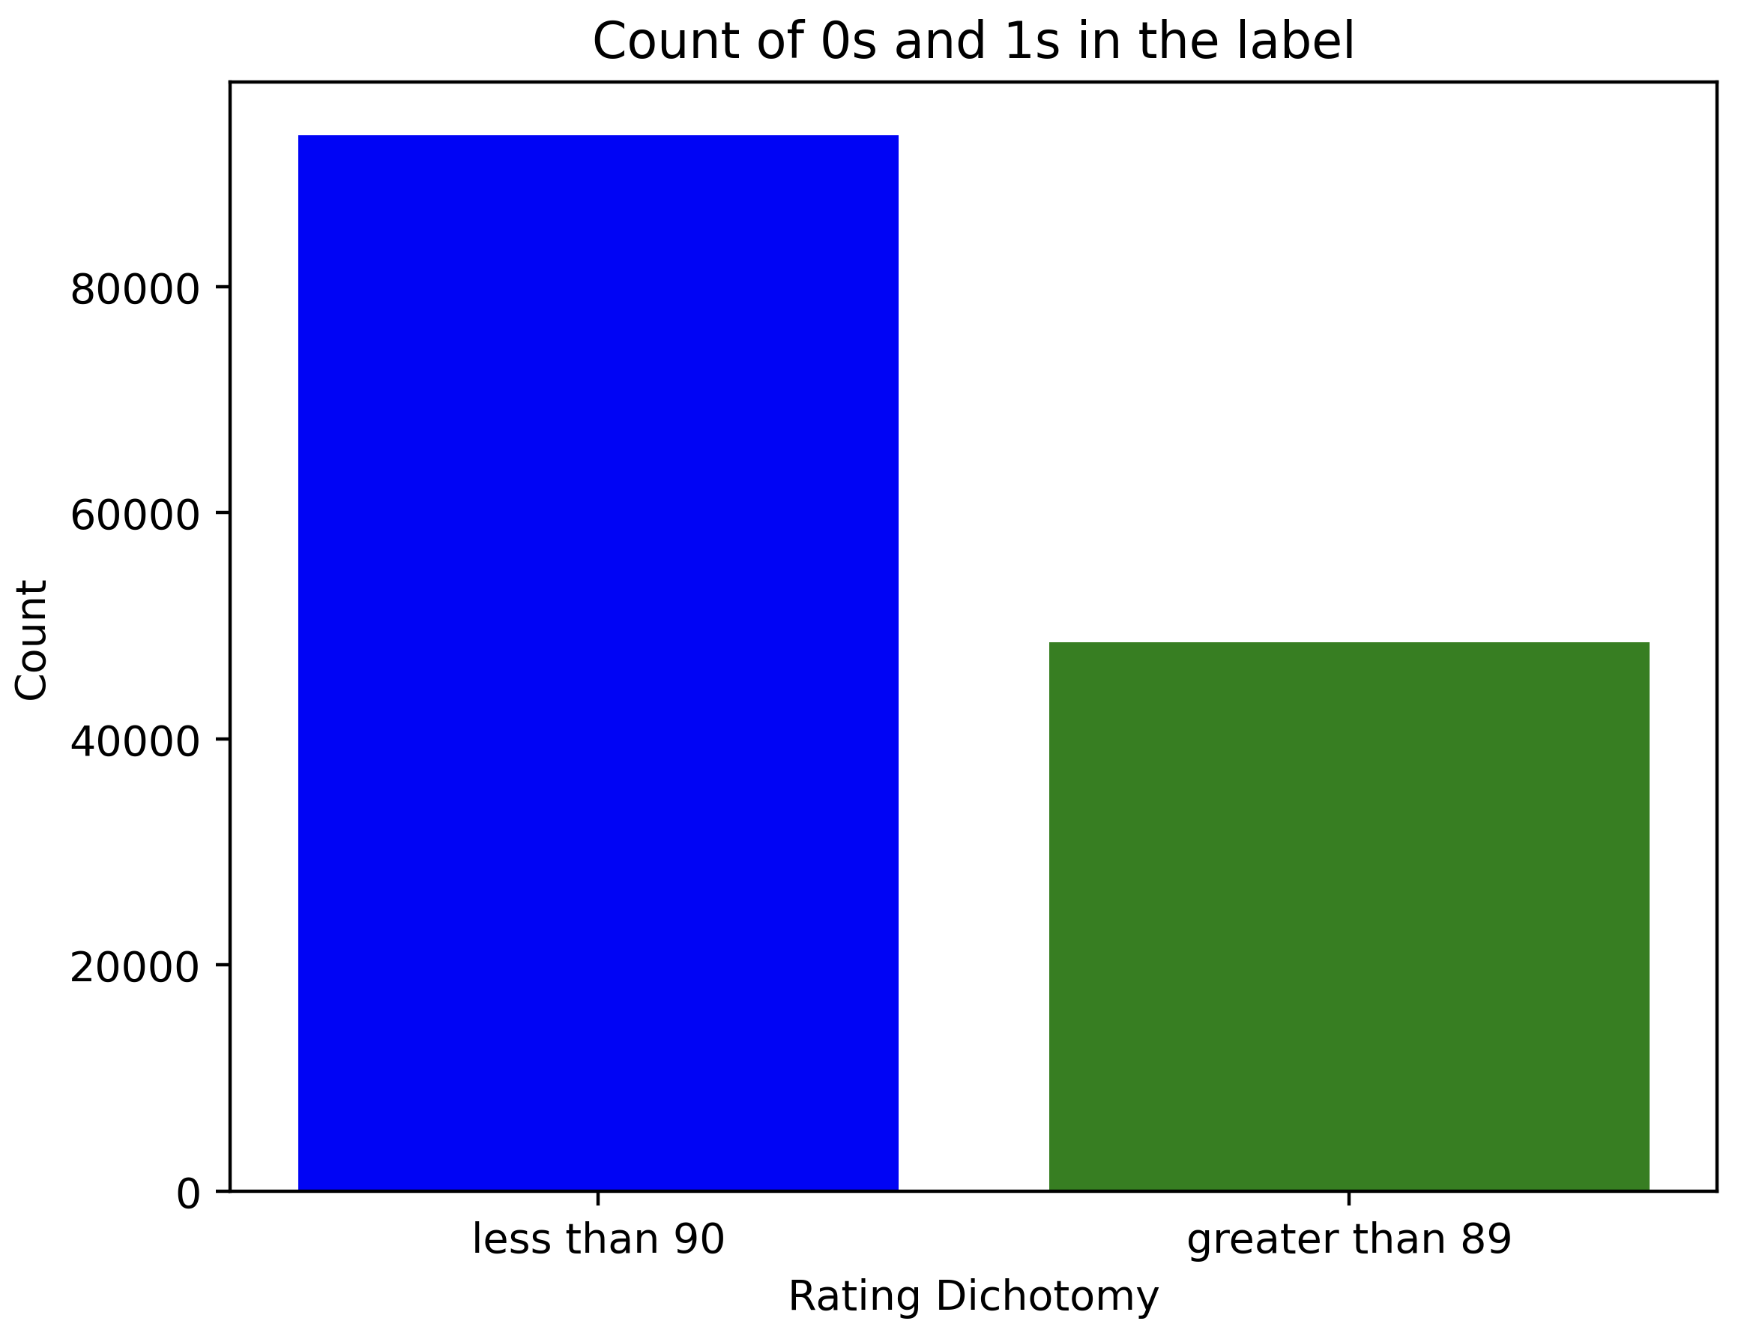
\includegraphics[scale=0.3]{img/dis.png}
\caption{The bar plot of the distribution of this dichotomized rating}
\label{Fig12: dis}
\end{figure}
\cite{chenyu} defined a function to fix all reviews of the same length of 100. This is realized by padding short reviews with prefixed zeros or truncating long reviews at the tail. It's common to align all documents with the same length in natural language understanding. The first reason is that stochastic gradient descent in backpropagation usually uses one batch of datasets, which involves a lot of matrix multiplication and matrix pairwise operations. Different sequence lengths in one batch probably complicate the implementations and further slow the training. The second reason is that some natural language models even require input sequence lengths to be the same. In his implementation, he didn't remove stop words because he thought the first layer of his attention-based models was trained to select sentiment words. He didn't stem words because he concluded that different base word forms in wine reviews sometimes carry different sentiments. For instance, \textit{"acidity"} means positive in a review, \textit{"The acidity of this wine is balanced"}. However, \textit{"acidic"} means negative in a review, \textit{"This wine is too acidic"}. So, stemming all words decreases the test accuracy. 

After preprocessing reviews, \cite{chenyu} split the dataset into training, validation, and testing sets. The split ratio is 18:1:1. Then, three sets were converted into tensor format with \href{https://pytorch.org/docs/stable/generated/torch.from_numpy.html}{torch.from\_numpy}. He used \href{https://pytorch.org/tutorials/beginner/basics/data_tutorial.html}{DataLoader} to create a batch of 64 and shuffle each batch. 

After dealing with data, he defined a few Python classes to implement his AMIC. The first class is \textbf{SelfAttention} inherited from a base class named \textbf{nn.Module}. This base class serves all neural network modules, and all self-defined neural network methods should subclass it. This \textbf{SelfAttention} class uses an 8-head self-attention method that includes \textit{query}, \textit{key}, and \textit{value}. In natural language understanding, a \textit{query} usually refers to a task or question. A \textit{key} refers to the relevant important information to this \textit{query}. A \textit{value} refers to a corpus of documents, books, articles, and so on. The second class is \textbf{tiedLinear} inherited from \textbf{nn.Module}. This class is defined to reduce model complexity and prevent overfitting using the same weight matrix for the input and output layers. The third class is \textbf{PositionalEncoding}. This class adds the word position information into the word embeddings. This is critical and helpful for sequence data, especially for natural language understanding. The fifth class is \textbf{Mask\_block}. This class incorporates class \textbf{SelfAttention}, \textbf{tiedLinear}, \href{https://pytorch.org/docs/stable/generated/torch.nn.Dropout.html}{dropout} for regularization, and $p_1 \;\&\; p_2$ for penalty terms. The sixth class is \textbf{Senitment\_block}. This uses \textbf{SelfAttention}, \textbf{tiedLinear}, \textbf{PositionalEncoding}, and dropout regularization to compute word-level context-based attentions. The last layer calculates the average word sentiment scores in one review to predict the document-level sentiment. The seventh class is \textbf{Synthesizer}. This class synthesizes the \textbf{SelfAttention} and \textbf{tiedLinear}. The eighth class is \textbf{Embeds}. This class incorporates the \textbf{PositionalEncoding} information into the pre-trained input word embeddings.

After defining all the above essential classes, he defined the number of layers to be 2, the number of heads to be 10, the dimension of hidden layers to be 300, and fixed the random seeds for reproducibility. Then, he initialized objects of \textbf{Embeds, Snetiment\_block, Mask\_block, and Synthesizer}. Now, he needed to set up the hyperparameters in the training process. There are many hyperparameters in this model. In his training process, he used the most popular gradient-based optimization algorithm for his stochastic objective function, \href{https://pytorch.org/docs/stable/generated/torch.optim.Adam.html}{Adam}. \cite{kingma2014adam} proposed Adam, and their paper has been cited 164,147. Adam is very well-known for its fast convergence and adaptive learning rating. \cite{chenyu} set up 0.0002 learning rates for four objects. He also used \href{https://pytorch.org/docs/stable/generated/torch.optim.lr_scheduler.StepLR.html}{scheduler} function to decay learning rates of parameters by gamma every a few steps. Unfortunately, the default numbers for these hyperparameters in his code didn't reproduce his 89.26\% test accuracy reported in his paper. Then, I spent some time tuning these hyperparameters to reach his results. I tuned the step size to be 2 and the gamma to be 0.65 in the above \href{https://pytorch.org/docs/stable/generated/torch.optim.lr_scheduler.StepLR.html}{scheduler}. \cite{chenyu} chose \href{https://pytorch.org/docs/stable/generated/torch.nn.BCELoss.html}{Binary Cross Entropy} to calculate the loss between predictions and true labels. \cite{chenyu} used 10 epochs in his code. However, I found that 10 epochs were insufficient because, at the 10th epoch, the rate of training accuracy wasn't flat. I set up 15 epochs for this training process. After discussing with \cite{chenyu} that I couldn't reproduce his reported accuracy, he told me that $c_1$ in the first penalty term was an important hyperparameter that greatly affected the performance. The default training codes that he sent to me had a few bugs. The bug occurred in the \textbf{Sentiment\_block} object. The definition of this object has three outputs in the forward function. However, in his code, he only specified one output to receive the outcome from this object. Because his training code is very long in one code chunk, Python only threw an error that the dimensions didn't match between one matrix and another, I spent a long time locating this bug by printing the intermediate matrix dimensions. The model was saved whenever the validation loss of this model was lower than a predefined constant. \cite{chenyu} didn't describe what this predefined constant is. After reviewing his codes, I assume this predefined constant is the best training model loss he has reached. In neural network training, plotting the changes in accuracy and loss against epochs is common and important. However, \cite{chenyu} didn't do this in his shared code. I added a new line of codes to record each epoch's validation accuracy, validation loss, and training loss for plotting purposes. The whole training process took me 13 minutes to finish. I plotted the average validation accuracy for each epoch in figure \ref{Fig13: val}. I observed that the average validation accuracy increased sharply between Epoch 1 and Epoch 5. However, between Epoch 6 and Epoch 12, the average validation accuracy slowly increased. After Epoch 13, this accuracy stayed the same almost. I also plotted each epoch's average training and validation loss in figure \ref{Fig14: loss}. I observed that the validation loss decreased considerably before Epoch 4. After Epoch 5, it decreased very slowly and stayed the same. However, the training loss fluctuated very often.  
\begin{figure}[ht]
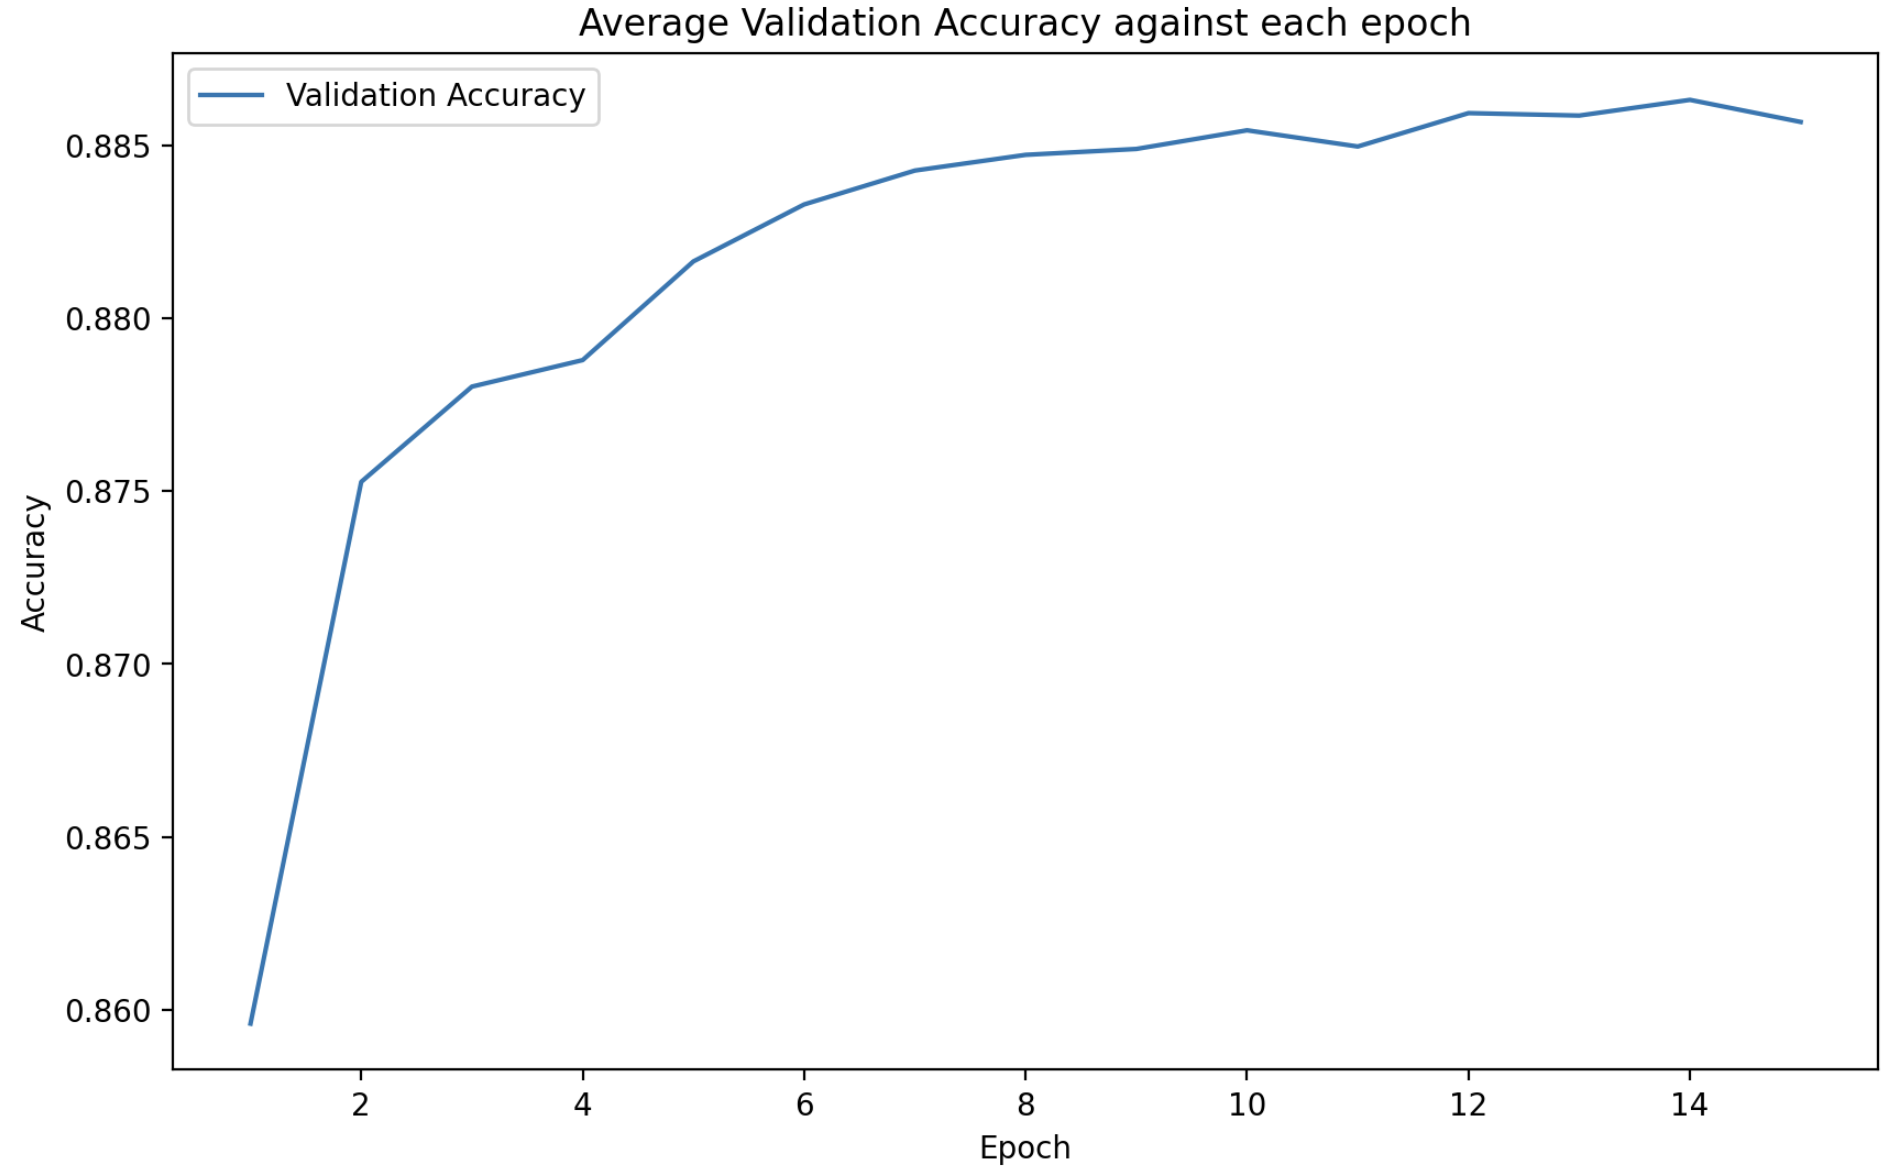
\includegraphics[scale=0.3]{img/val.png}
\caption{The average validation accuracy of each epoch}
\label{Fig13: val}
\end{figure}
\begin{figure}[ht]
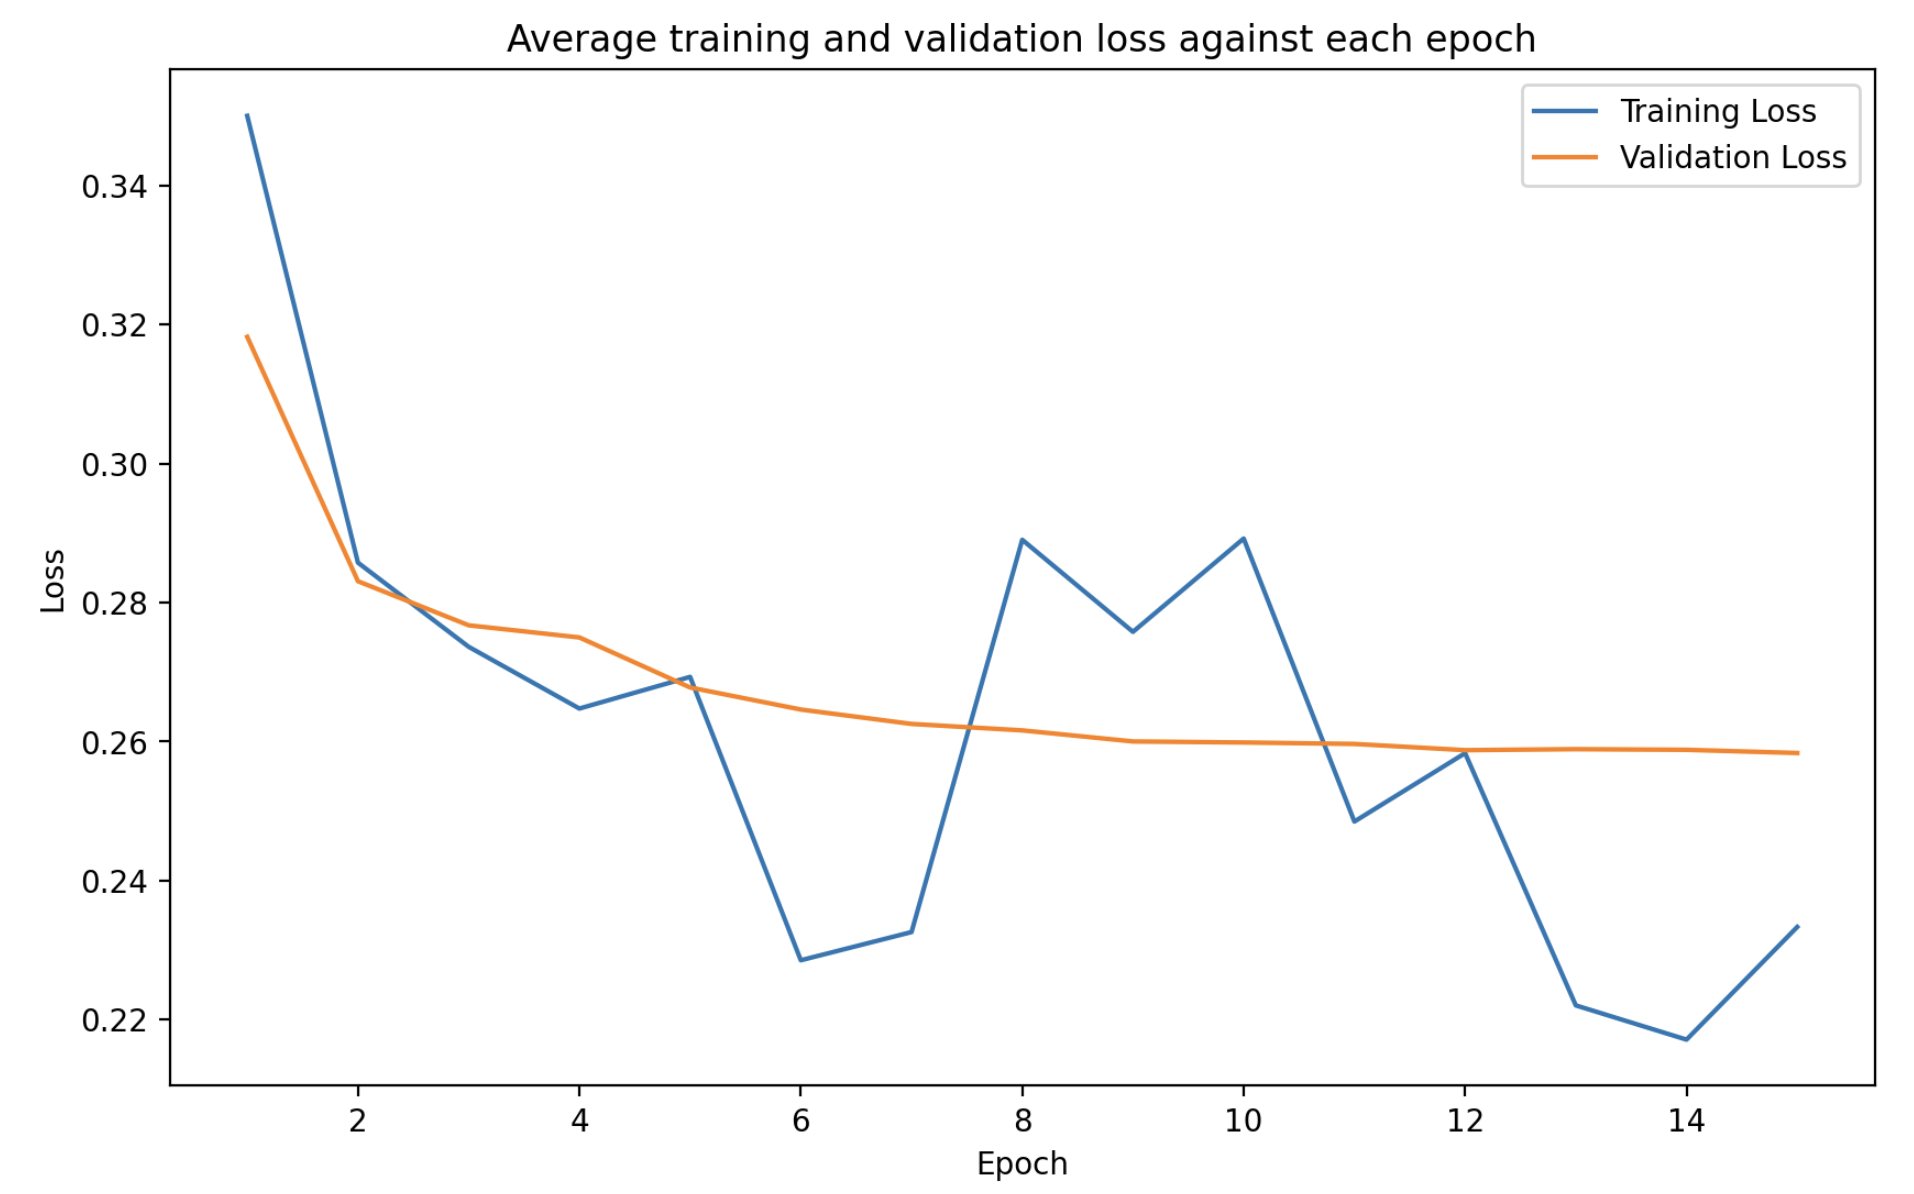
\includegraphics[scale=0.3]{img/loss.png}
\caption{The average training and val loss of each epoch}
\label{Fig14: loss}
\end{figure}
The final best saved model achieved 88.99\% training accuracy. It achieved 88.66\% validation accuracy. However, it only achieved 88.89\% test accuracy. My reproduction test accuracy, 88.89\%, is slightly lower than \cite{chenyu}'s reported one, 89.26\%. In addition to this implementation of AMIC, he conducted some inference analysis based on his trained models in his shared later codes. However, one code chunk must import external data files; most following codes depend on these files. He didn't share this with me. My edited version of \cite{chenyu}'s shared codes is available for further inspection at the colab \href{https://drive.google.com/file/d/181pkl3XwtB9SV06hoC_XT0XMyrzAlJoJ/view?usp=sharing}{Jupyter Notebook}.

Next, I reproduced his BERT model results because compared to CNN and BILSTM, BERT is the most state-of-the-art natural language understanding model. Unfortunately, \cite{chenyu} didn't share his BERT model codes. I had to write a BERT model from scratch and fine-tune it on the same \textit{wine review} dataset. In addition to all Python packages used in the AMIC model, the core package used to build a BERT model is the \href{https://huggingface.co/docs/transformers/index}{transformers package} developed by \href{https://huggingface.co/support}{the Hugging Face team}. I didn't apply the same preprocessing procedures that \cite{chenyu} applied to his AMIC model. Instead, I applied the most basic pre-trained BERT tokenizer, \href{https://huggingface.co/bert-base-uncased}{bert-base-uncased}, to the \textit{wine reviews}. \textit{bert-base-uncased} proposed by \cite{DBLP:journals/corr/abs-1810-04805} was pre-trained on a large corpus of English texts in a self-supervised way and doesn't differentiate cases. This tokenizer produces two parts for the training process. One part is \textit{input\_ids}, and another is \textit{attention\_masks}. I split the data into training, validation, and testing with the same ratio and random seed used in AMIC to ensure the splitting is the same as AMIC. Then I applied \textit{TensorDataset} and \textit{DataLoader} to prepare them for training. I shuffle each batch using \textit{RandomSampler} and \textit{SequentialSampler}. The batch size is 64, the same as AMIC. I used \href{https://pytorch.org/docs/stable/generated/torch.optim.AdamW.html}{AdamW} with a learning rate, $2\times10^{-5}$, as the optimization algorithm. I used \href{https://pytorch.org/docs/stable/generated/torch.nn.BCEWithLogitsLoss.html}{BCEWithLogitsLoss} as the loss function. This loss function is more numerically stable by combining a sigmoid layer with a BCELoss function into one class. Because this is a binary classification task, I used \href{https://huggingface.co/transformers/v3.0.2/model_doc/bert.html#bertforsequenceclassification}{BertForSequenceClassification} class to initialize the model with the \textit{bert-base-uncased} and set \textit{num\_labels} equal to one. I used \href{https://pytorch.org/docs/stable/generated/torch.nn.utils.clip_grad_norm_.html}{"torch.nn.utils.clip\_grad\_norm\_"} to cut off the gradient of the model parameters during training. This can prevent them from exploding. This ensures training is stable. I only used 2 epochs for training because the validation loss started decreasing from the second epoch. I used the same platform, colab, resources, T4 GPU, and high-Ram. It took 1 hour and 4 minutes to finish. I plotted the validation accuracy, loss, and training loss in figure \ref{Fig15: bert_acc} and figure \ref{Fig16: bert_loss}. The validation accuracy decreased from Epoch One to Epoch Two in the figure \ref{Fig15: bert_acc}. The validation loss increased from Epoch One to Epoch Two in the figure \ref{Fig16: bert_loss}. I applied the trained model to the test set and found that the test accuracy was 88.75\%. This 88.75\% test accuracy is also slightly lower than the test accuracy \cite{chenyu} reported, 89.12\%. However, my reproduced AMIC test accuracy, 88.89\%, is higher than my defined BERT test accuracy, 88.75\%, though they are essentially very close. For a more robust comparison result, k-fold cross-validation is desirable because it gives us the mean and standard deviation of test accuracy. However, I didn't do it because \cite{chenyu} didn't apply it in his original code. He only reported the best model he had reached, and so did I. From this comparison, I found the biggest advantage of AMIC was it provided word-level interpretability and achieved comparable predictive performance with much less running time and resources. My code for the BERT model is available for further reproduction and inspection at the colab \href{https://colab.research.google.com/drive/1oZDrhat5LBbGv2ug-e2SBBOMlj6LoNyu?usp=sharing}{Jupyter Notebook}.    
\begin{figure}[ht]
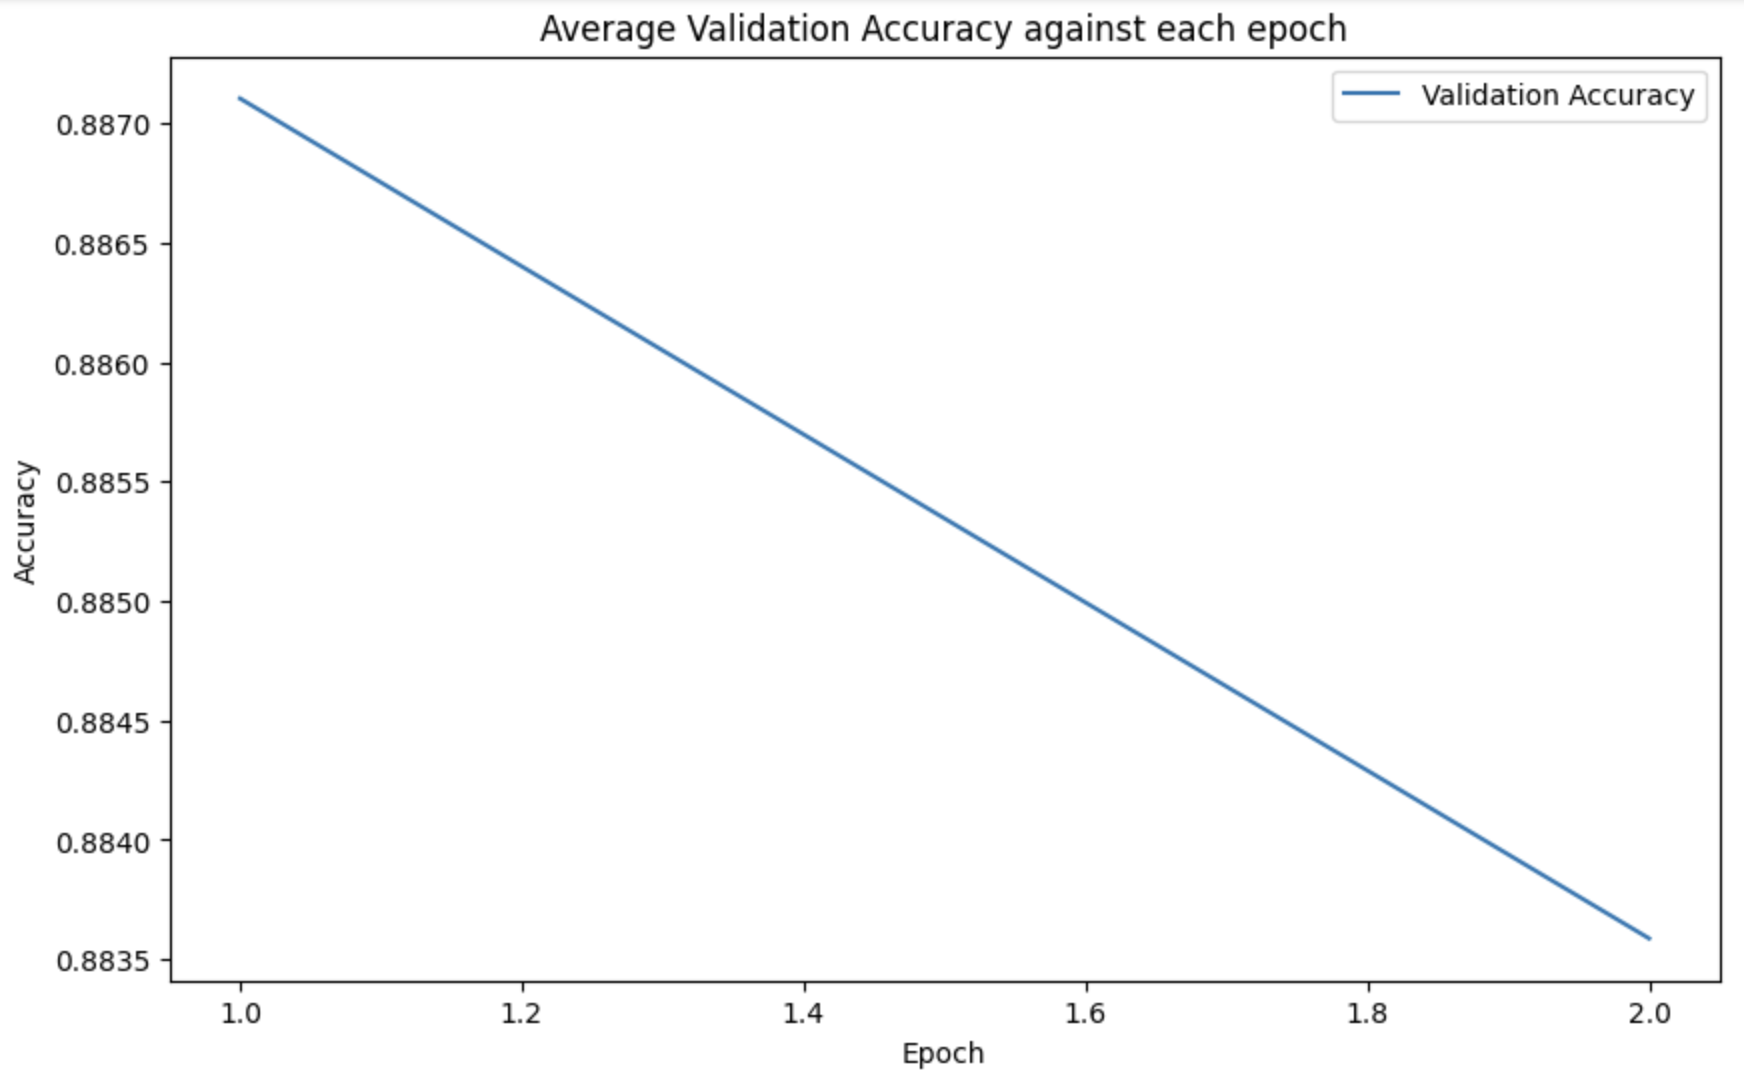
\includegraphics[scale=0.3]{img/bert_acc.png}
\caption{The average validation accuracy of each epoch}
\label{Fig15: bert_acc}
\end{figure}
\begin{figure}[ht]
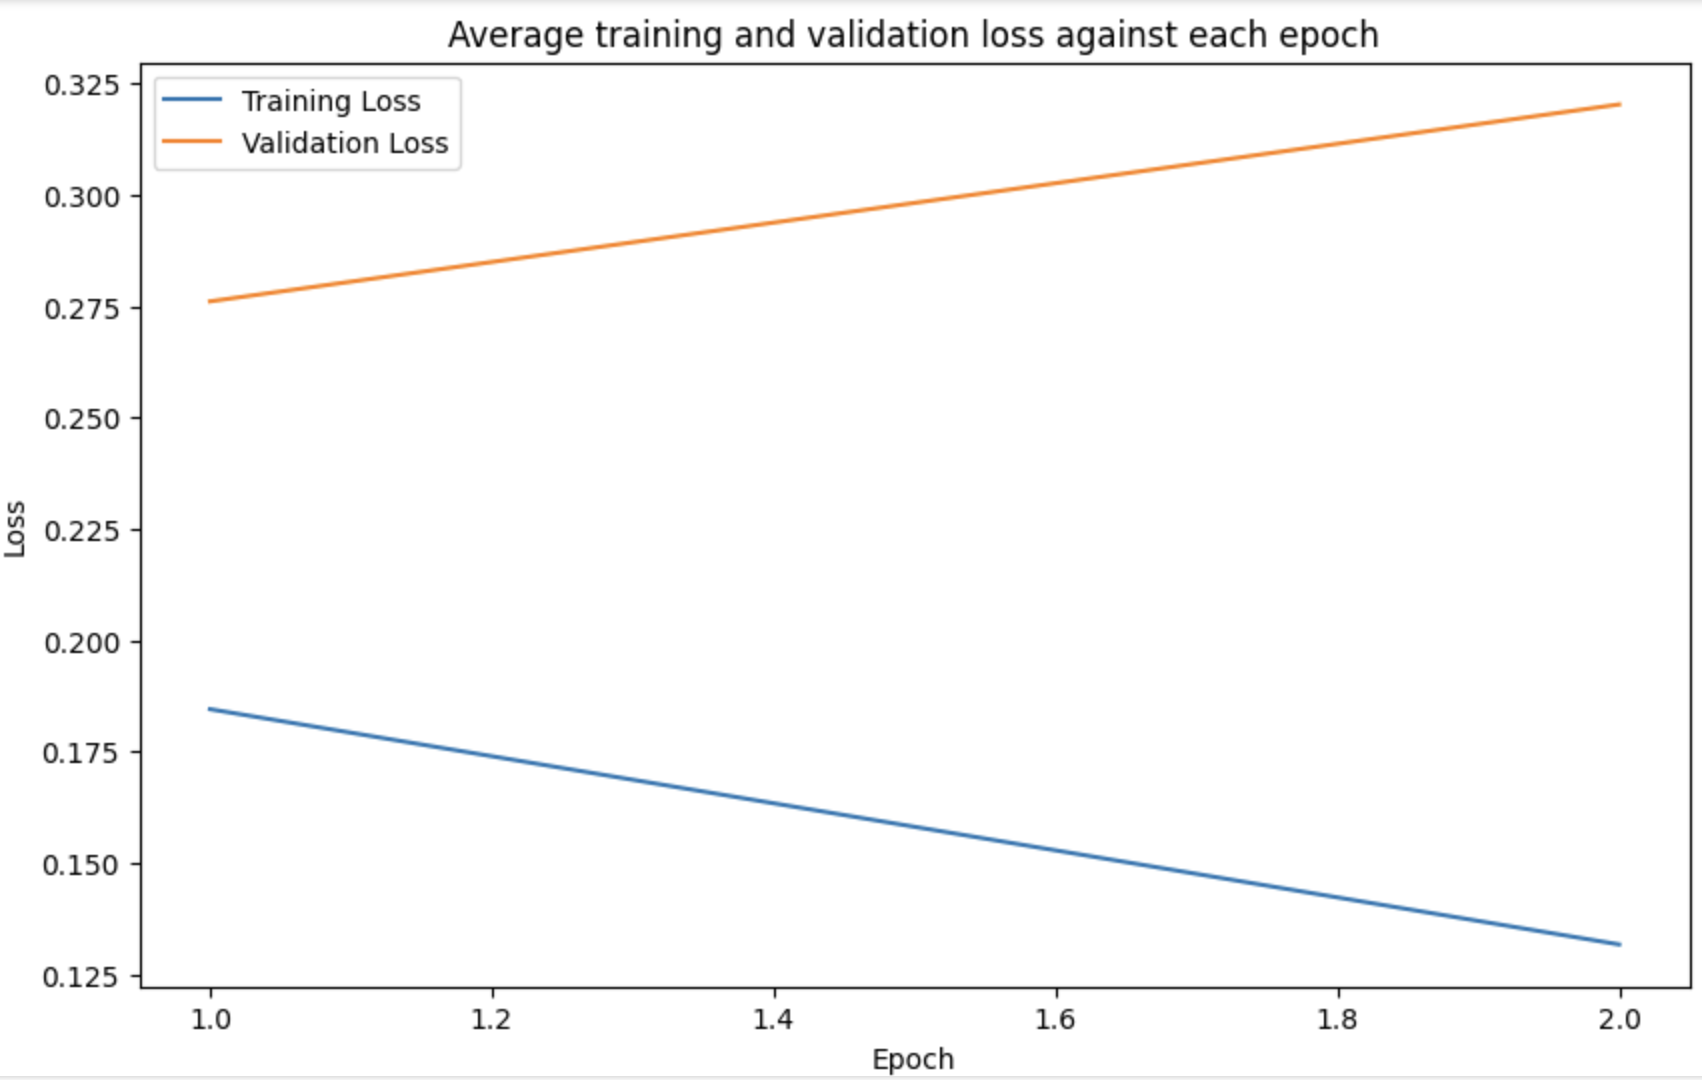
\includegraphics[scale=0.3]{img/bert_loss.png}
\caption{The average training and val loss of each epoch}
\label{Fig16: bert_loss}
\end{figure}

\section{Future Directions}
This section explored some future directions beyond \cite{chenyu}'s work. There are many ways to extend his work. The most straightforward direction is that I inspect if his method suffers from learning some surface-level patterns to make sentiment analysis. My idea was inspired by the \cite{DBLP:journals/corr/abs-1909-12434}' work. As I discussed in section two, they found that some natural language understanding models usually classify sentiments by spurious textures, and they proposed a method to augment the original data with counterfactual instances to retrain models. \cite{DBLP:journals/corr/abs-1909-12434} published their IMDB movie review dataset for the sentiment analysis at their \href{https://github.com/acmi-lab/counterfactually-augmented-data/tree/master}{GitHub}. I pulled their original, revised, and combined data from their GitHub to experiment with them on the \cite{chenyu}'s AMIC. 

I used the same platform, Google Colab, and their T4 GPU for this experiment. \cite{DBLP:journals/corr/abs-1909-12434} have split their IMDB dataset into training, validation, and testing sets. The original training set has 1707 observations, the original validation set has 245 observations, and the original test set has 488 observations. I printed the head of this IMDB dataset in my Jupyter notebook and placed the screenshot of it in the figure \ref{Fig17: imdb}.
\begin{figure}[ht]
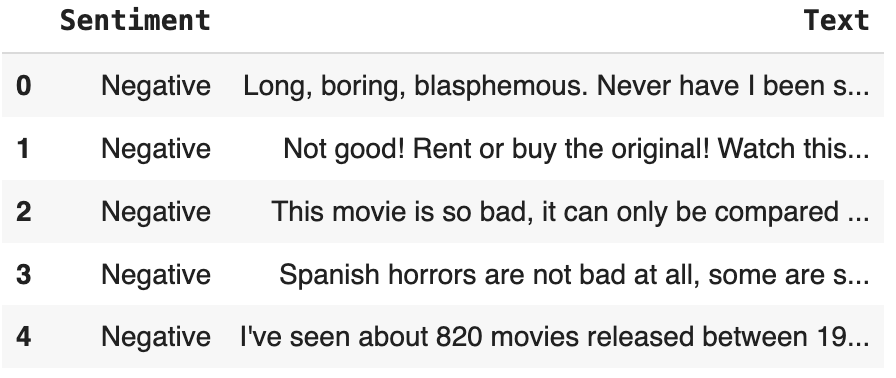
\includegraphics[scale=0.7]{img/imdb.png}
\caption{The head of IMDB dataset}
\label{Fig17: imdb}
\end{figure}
Then, I applied all the same preprocessing procedures, including tokenizing reviews, creating word embeddings for unique words, removing words, and calculating review lengths. I plotted a bar plot to inspect the ratio between negative and positive sentiments in the original IMDB dataset in Figure \ref{Fig18: imdbsent}. The ratio is 1:1, an ideal situation for a binary classification. 
\begin{figure}[ht]
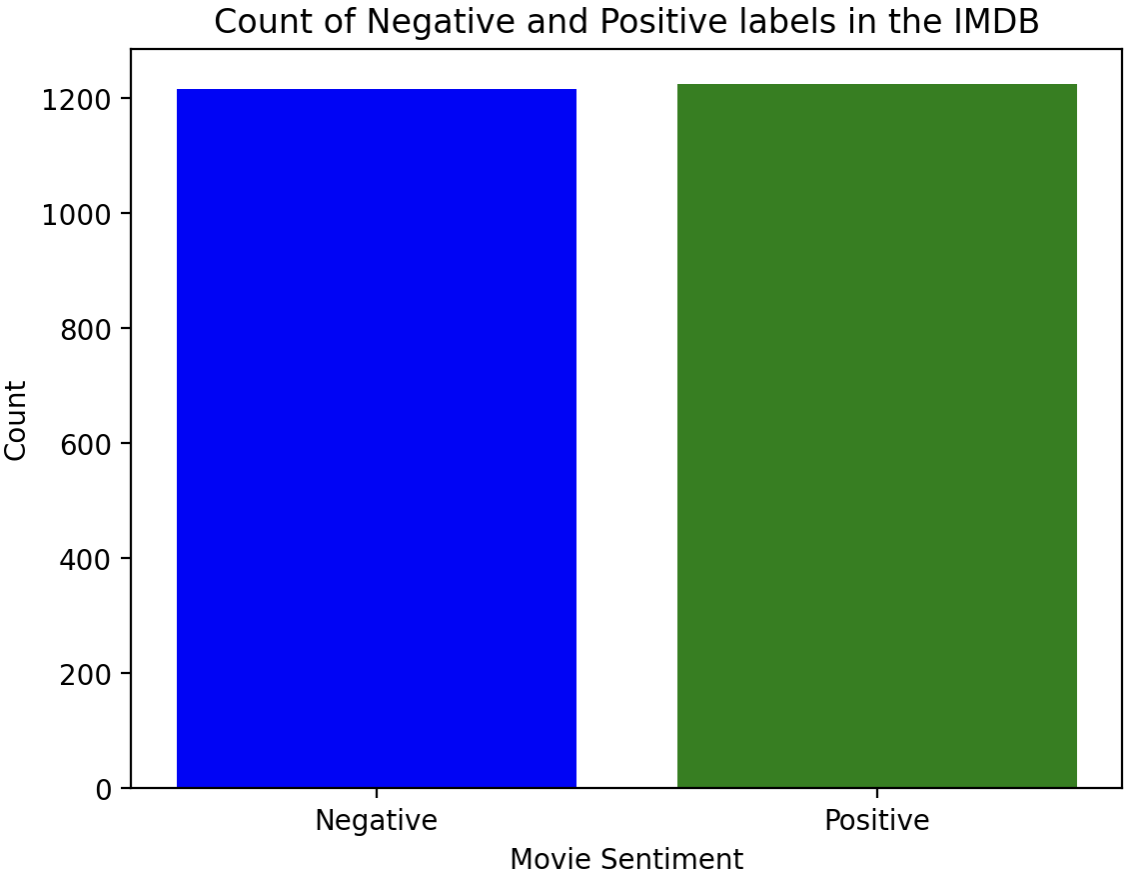
\includegraphics[scale=0.3]{img/imdbsent.png}
\caption{The bar plot of negative and positive sentiments in the original IMDB}
\label{Fig18: imdbsent}
\end{figure}
I increased the padded length for all movie reviews to 350 instead of 100 in \cite{chenyu}'s \textit{wine review} because this IMDB dataset has much fewer observations than \textit{wine review}. I used the same \textit{TensorDataset} and \textit{DataLoader} to prepare the IMDB data for training in PyTorch. In the \textit{DataLoader}, I increased the batch size to 128 instead of 64 after tuning the batch size parameter. The size of the final embedding matrix for all words is 21,196 by 300. I applied all the same \cite{chenyu}'s defined classes in his AMIC to the IMDB data. However, I encountered a big challenge during the training process. Since the data was changed completely, the original default hyperparameters achieved around 50\% validation accuracy, a random guess. Then, I spent at least 8 hours tuning the hyperparameters of AMIC, including four learning rates, step sizes, \href{https://pytorch.org/docs/stable/generated/torch.optim.lr_scheduler.StepLR.html}{gamma} (decay ratio), $c_1, c_2$ penalty constants, and the number of epochs. I set up \textbf{Embeds}'s learning rate to be 0.05, \textbf{Sentiment\_block}'s learning rate to be 0.09, \textbf{Mask\_block}'s learning rate to be 0.07, and \textbf{Synthesizer}'s learning rate to be 0.06. I set up all the learning rates to decay by 0.7 for every 1-step size of each epoch. I set up 30 epochs in total. I set up the $c_1$ penalty constant to be 0.001. I changed the way I saved the best AMIC model during training. \cite{chenyu} saved the best model whenever the validation loss was lower than a predetermined constant. I found this way was a pitfall because a high validation accuracy could have either low or high validation loss. In light of this, I saved the best model whenever the validation accuracy was higher than 84\% because the validation accuracy is not stable as shown in the figure \ref{Fig19: imdbdev}, making me not to adopt an early stopping strategy. After about 2 minutes of training, I plotted the validation accuracy changes against each epoch and loss for the training and validation sets in the figure \ref{Fig19: imdbdev} and \ref{Fig20: imdbloss}. In the figure \ref{Fig19: imdbdev}, the validation accuracy kept increasing though fluctuating. In figure \ref{Fig20: imdbloss}, the training loss decreased sharply before Epoch 5 but decreased very slowly after Epoch 5. The validation loss decreased before Epoch 5 but increased after Epoch 5, which suggested this training may be overfitting. The final trained model achieved 97.9\% training accuracy, 78.91\% validation accuracy, and 77.6\% test accuracy. 
\begin{figure}[ht]
    \centering
    \begin{minipage}{0.45\textwidth}
        \centering
        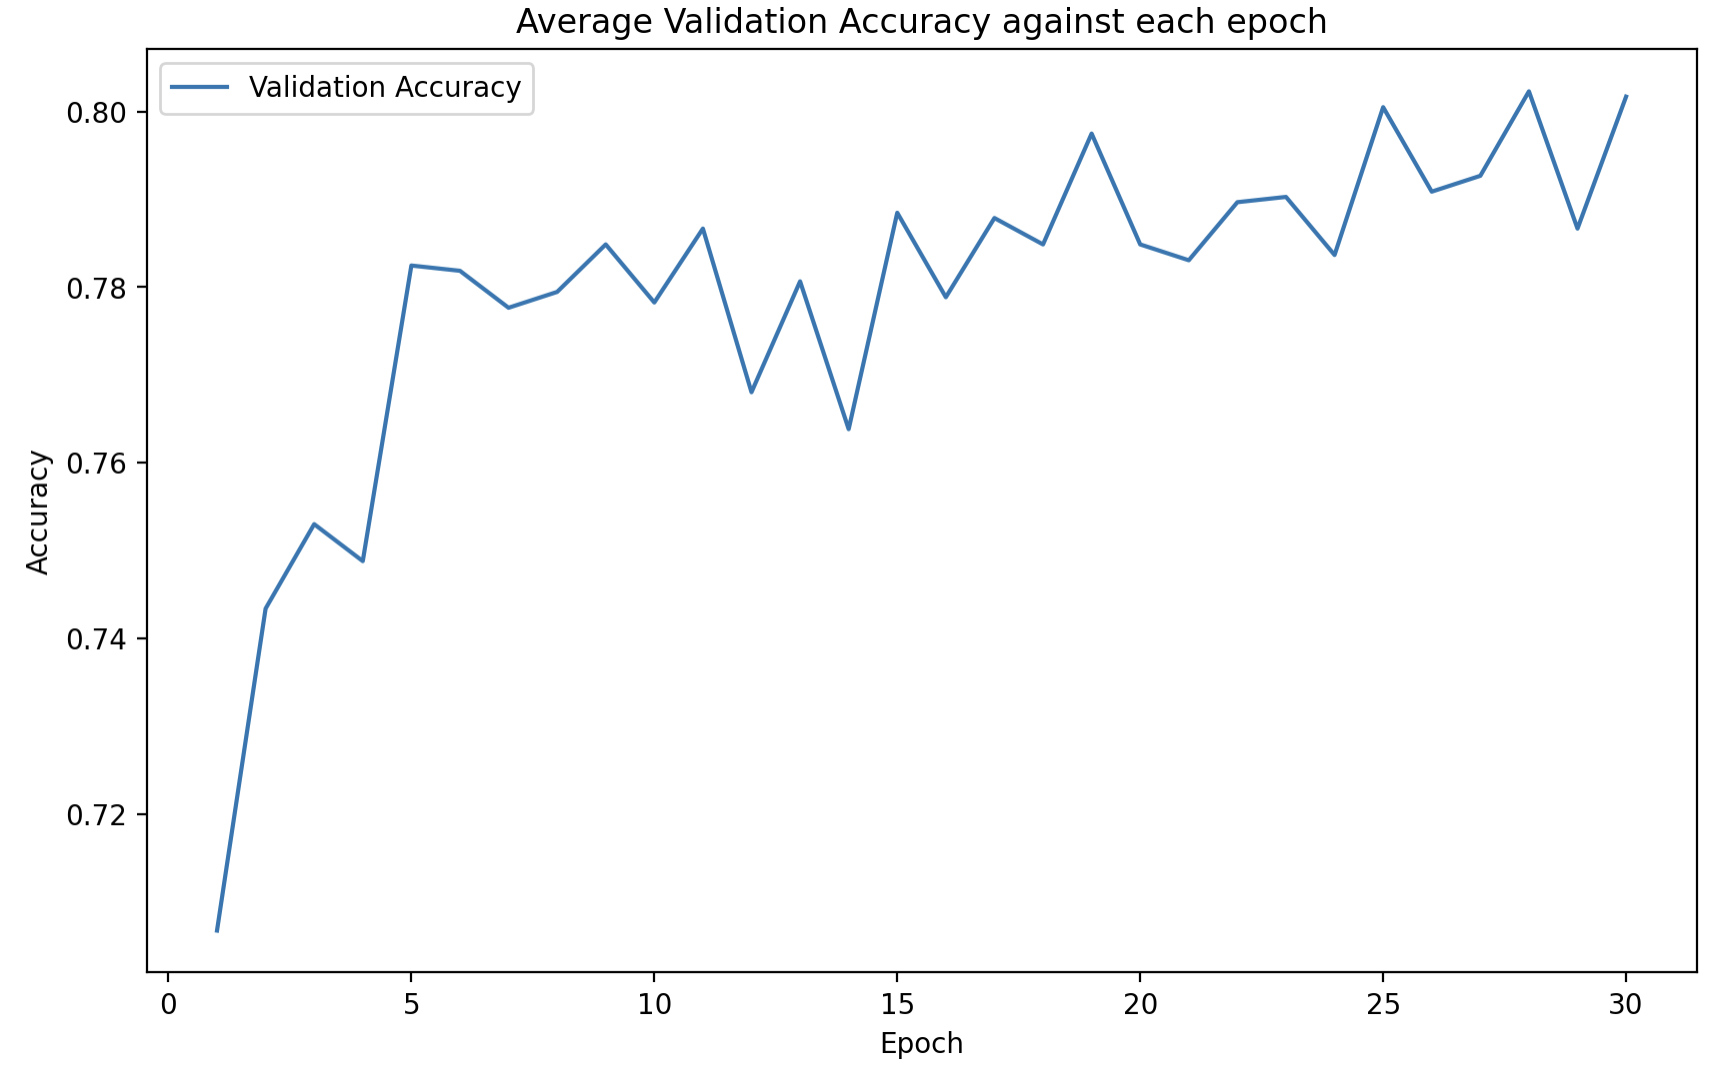
\includegraphics[width=\textwidth]{img/imdb_dev.png}
        \caption{Validation Accuracy on the original IMDB data}
        \label{Fig19: imdbdev}
    \end{minipage}
    \hfill
    \begin{minipage}{0.45\textwidth}
        \centering
        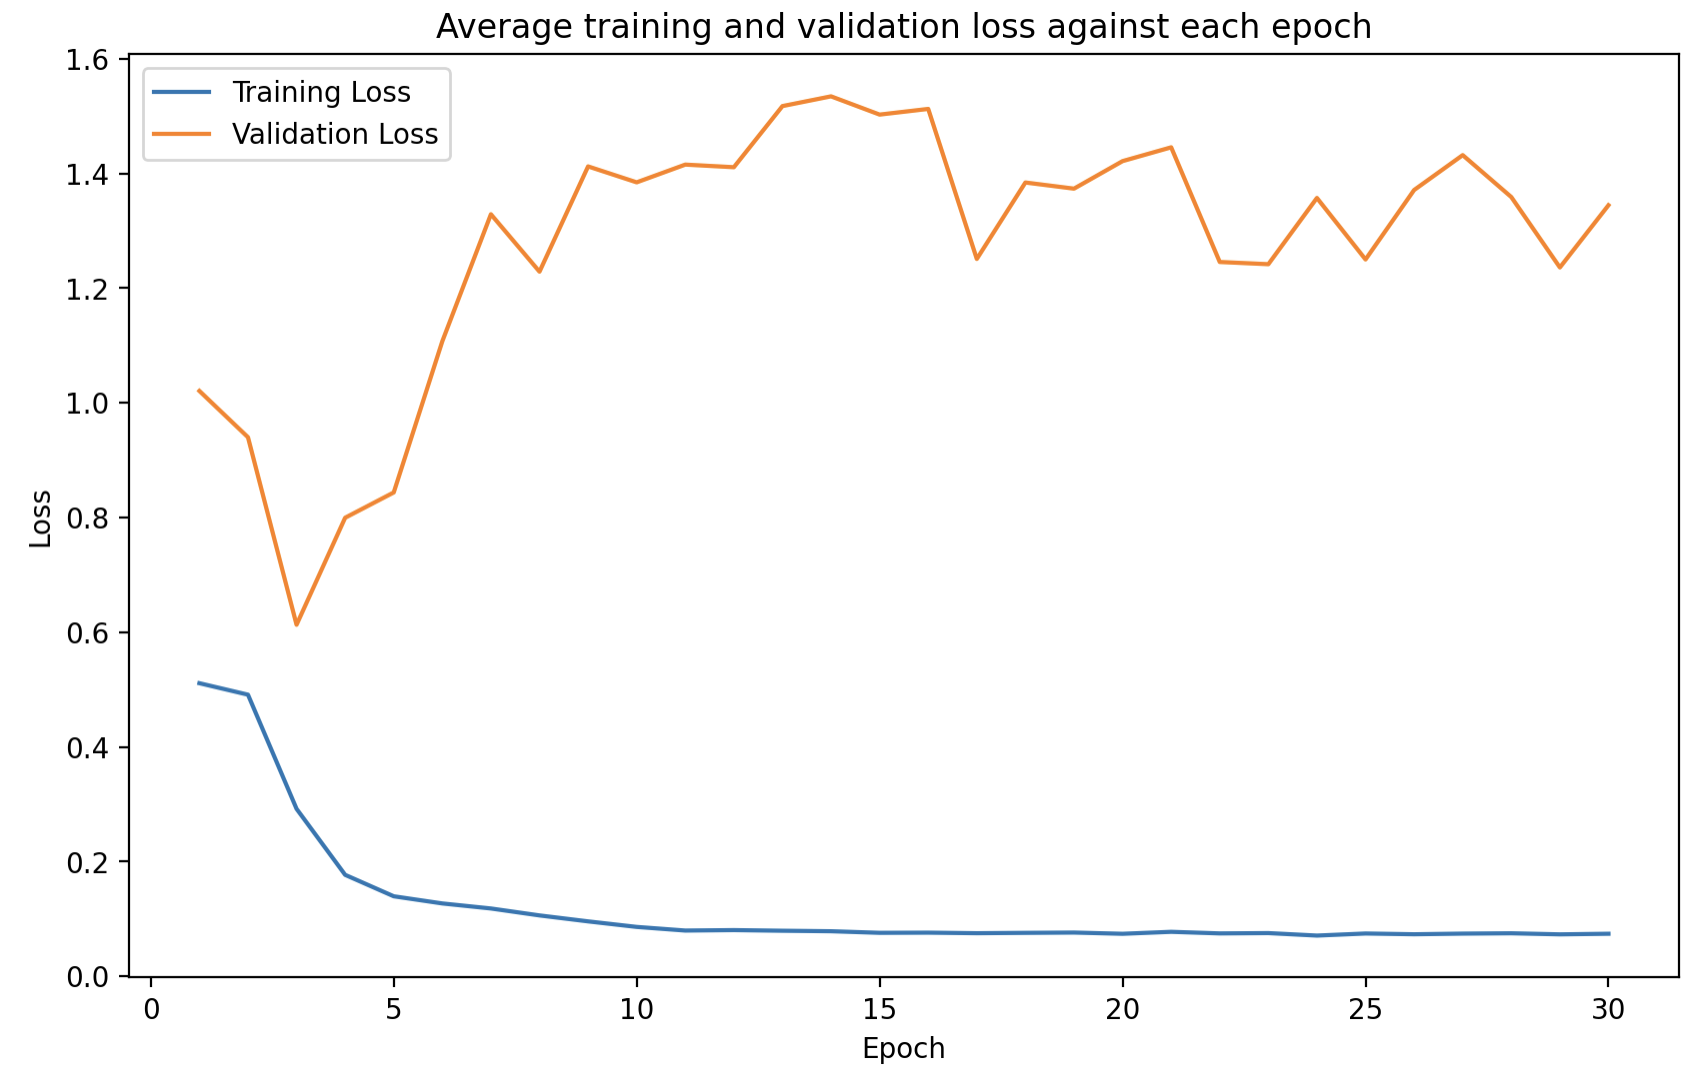
\includegraphics[width=\textwidth]{img/imdb_loss.png}
        \caption{Validation Loss on the original IMDB data}
        \label{Fig20: imdbloss}
    \end{minipage}
\end{figure}

Then I imported \href{https://github.com/acmi-lab/counterfactually-augmented-data/tree/master/sentiment/new}{the revised IMDB dataset}. The training set had 1,707 observations, the validation set had 245 observations, and the test set had 488 observations. I applied all the same preprocessing procedures to this revised dataset. However, the trained model on \href{https://github.com/acmi-lab/counterfactually-augmented-data/tree/master/sentiment/orig}{the original IMDB dataset} only achieved 52.7\% accuracy on the revised training set. \cite{DBLP:journals/corr/abs-1909-12434} predicted this phenomenon and proved it in the figure \ref{Fig21: orire}. For example, the Bi-LSTM model trained only on the original IMDB achieved 79.3\% accuracy but only 55.7\% accuracy on the revised IMDB. I can conclude that \cite{chenyu}'s AMIC still suffers from only learning the spurious textures in the sentiment analysis. 
\begin{figure}[ht]
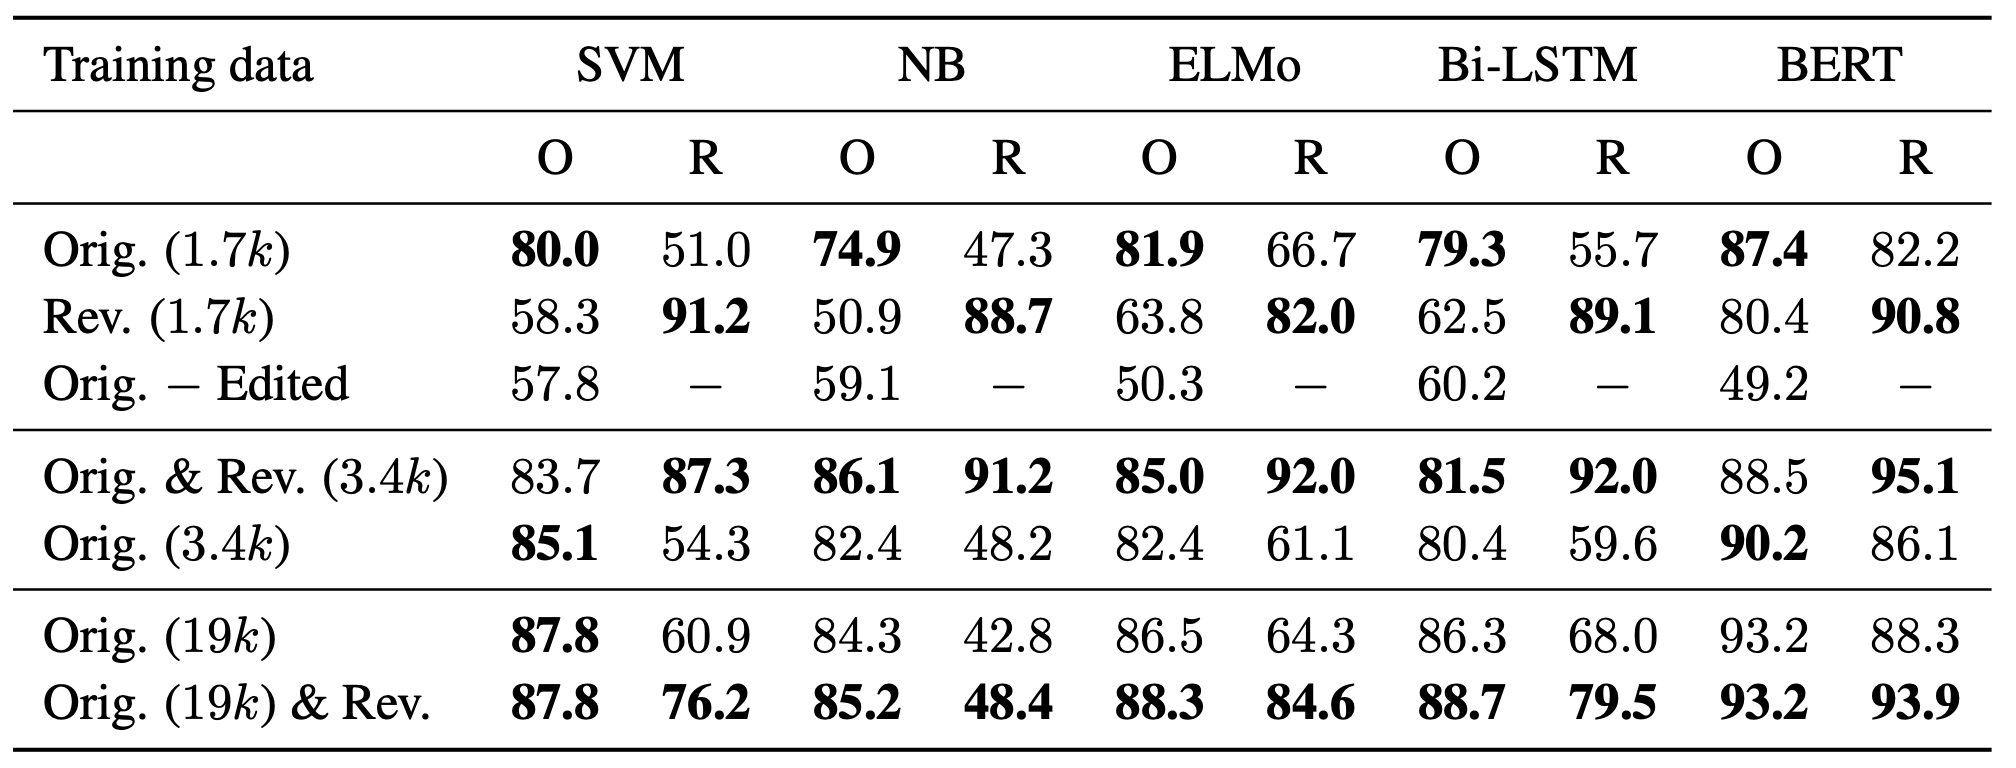
\includegraphics[scale=0.3]{img/orire.png}
\caption{The accuracy of IMDB on the original and revised data with different training data}
\label{Fig21: orire}
\end{figure}

Next, I investigated if models trained on the combined original and revised data improved the accuracy of the original and revised data separately. I trained the AMIC on the \href{https://github.com/acmi-lab/counterfactually-augmented-data/tree/master/sentiment/combined/paired}{combined data} by using all the same preprocessing procedures to the movie reviews. After tuning hyperparameters of AMIC models, I finally set up \textbf{Sentiment\_block}'s learning rate to be 0.07 and other classes' learning rates to be 0.05. The step size was one, and the gamma was 0.9. I used 30 epochs to train AMIC. I plotted the validation accuracy changes and loss in the figure \ref{Fig23: comacc} and \ref{Fig24: comloss}. This AMIC model learned a lot before Epoch 14, and the validation loss showed it started overfitting after Epoch 14.
\begin{figure}[ht]
    \centering
    \begin{minipage}{0.45\textwidth}
        \centering
        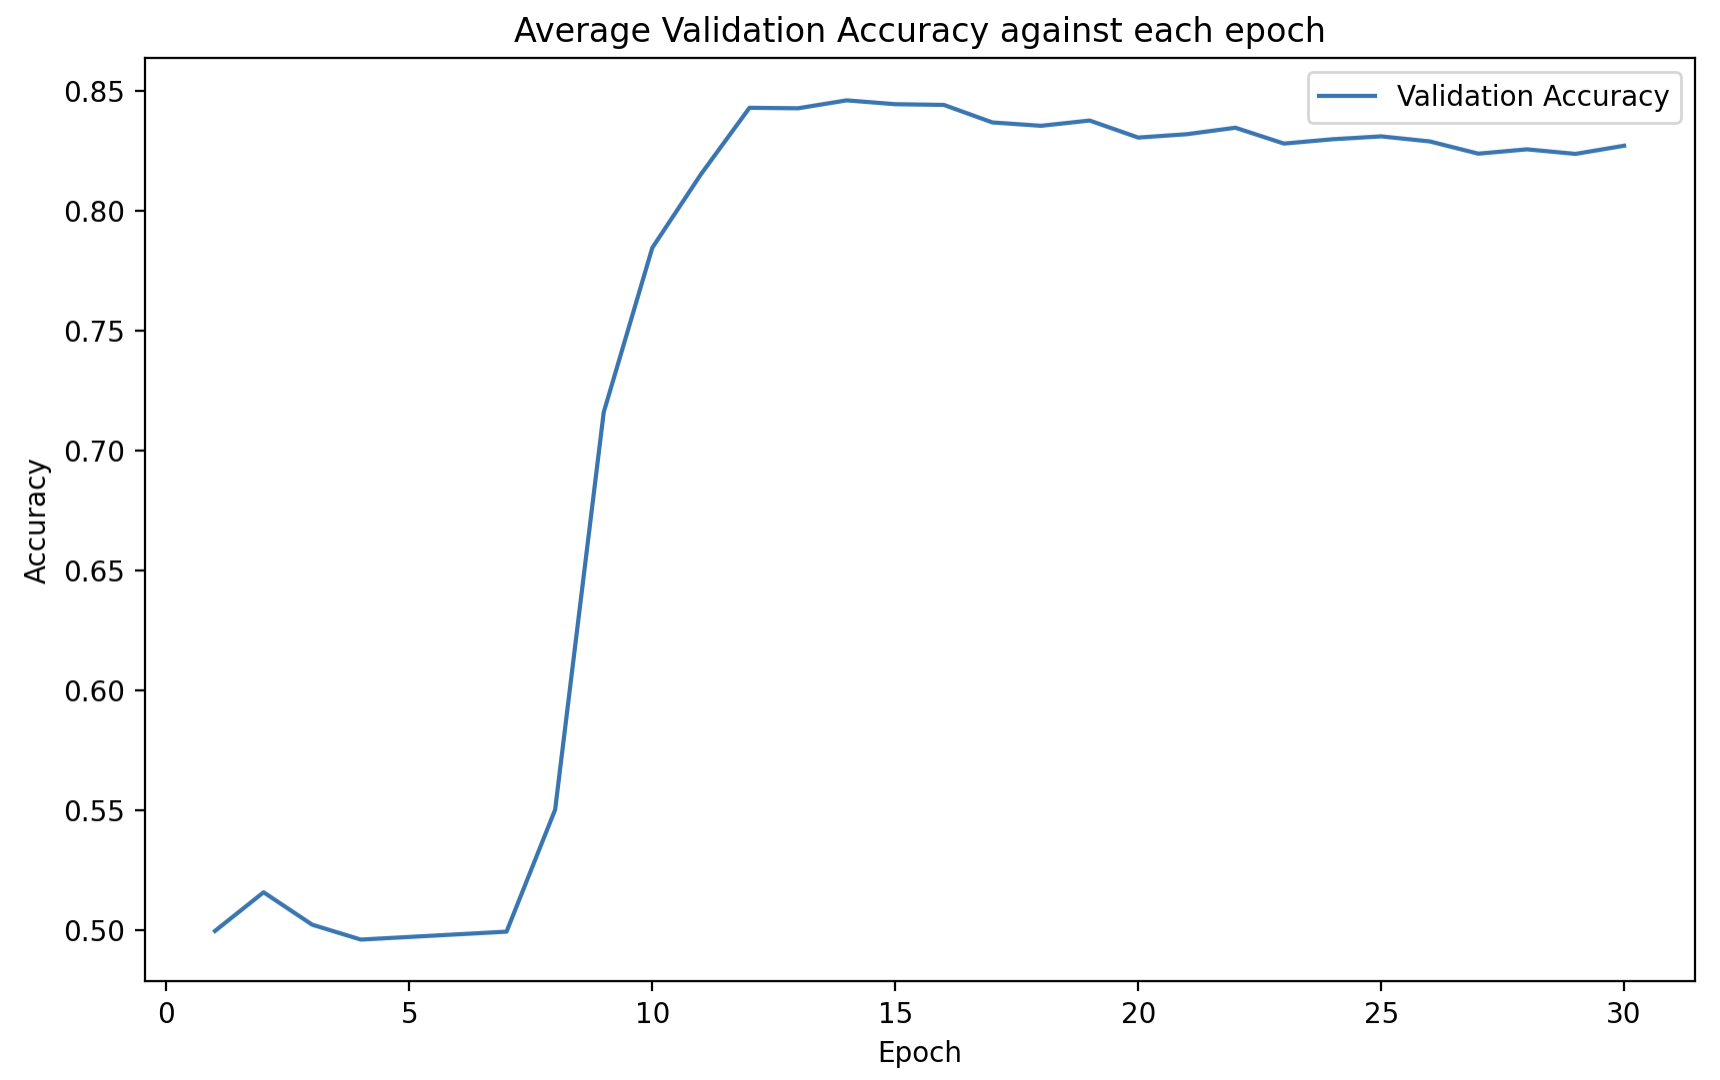
\includegraphics[width=\textwidth]{img/com_acc.png}
        \caption{Validation Accuracy on the combined data}
        \label{Fig23: comacc}
    \end{minipage}
    \hfill
    \begin{minipage}{0.45\textwidth}
        \centering
        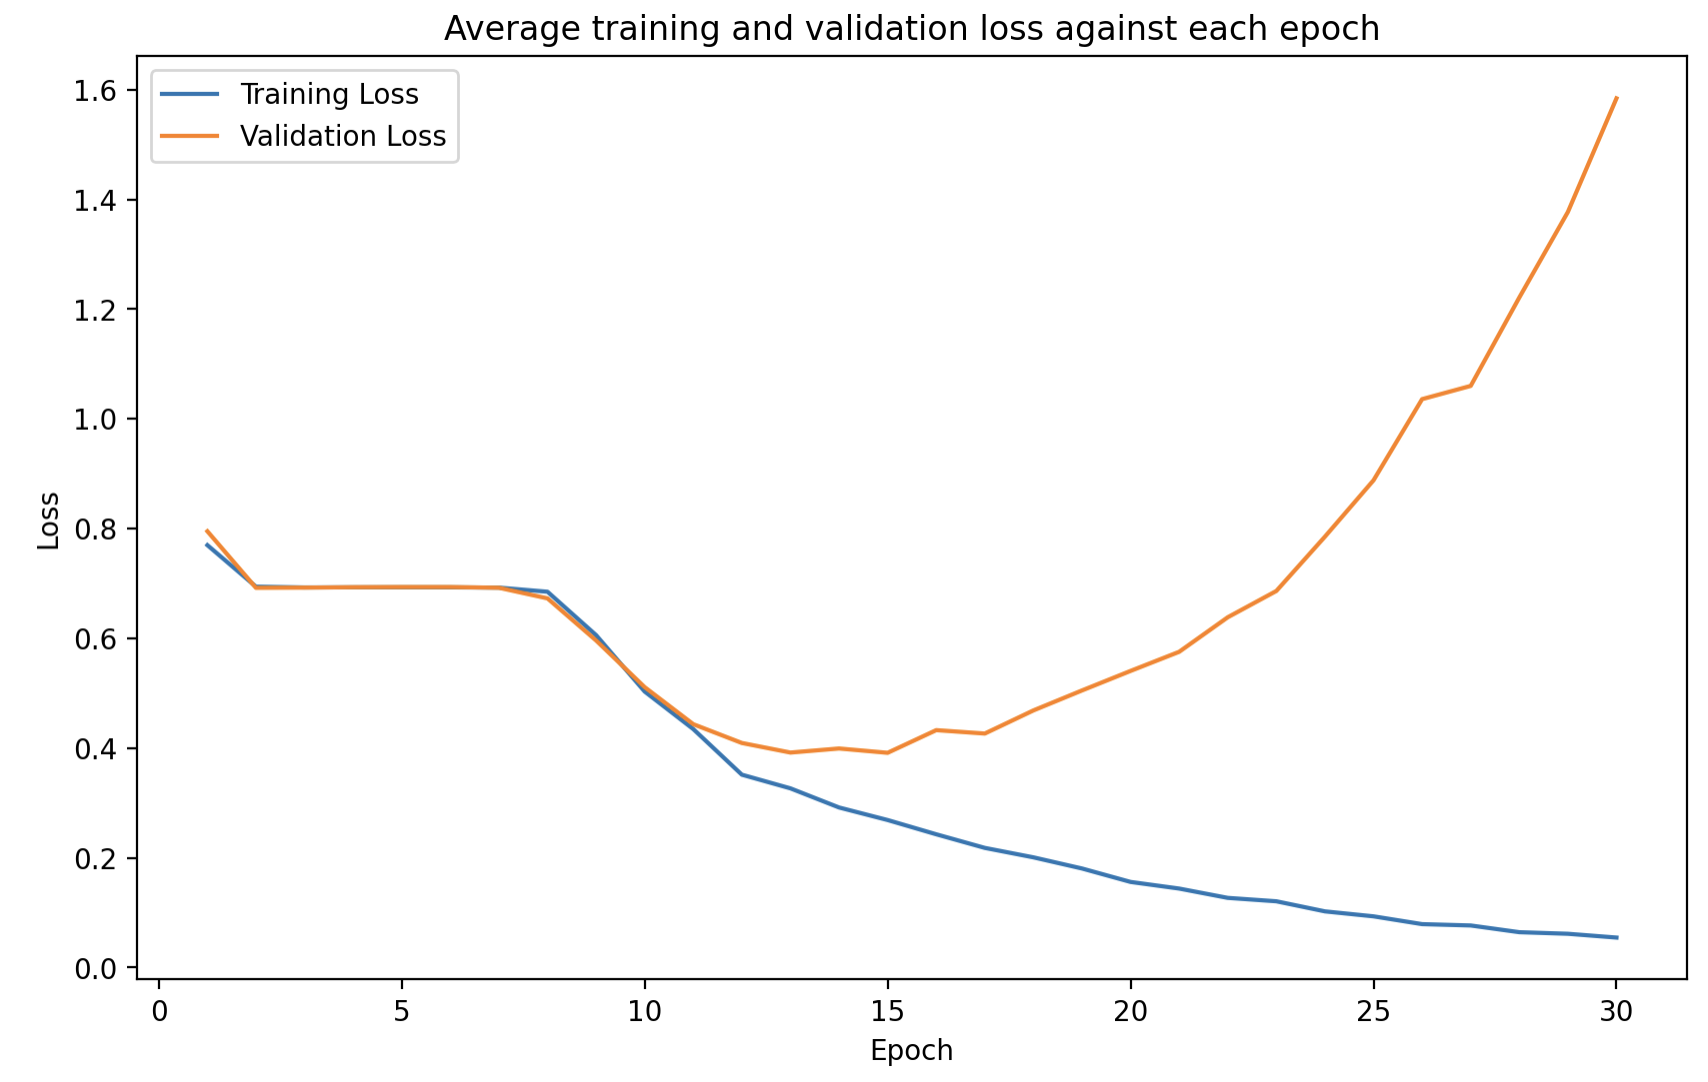
\includegraphics[width=\textwidth]{img/com_loss.png}
        \caption{Validation Loss on the combined data}
        \label{Fig24: comloss}
    \end{minipage}
\end{figure}

I made a table \ref{tab:comacc} to report the test accuracies trained on the original IMDB data, and the combined IMDB data with the AMIC model. In the table \ref{tab:comacc}, "O" represents the original and "R" represents the revised. The AMIC model trained on the original achieved 77.6\% test accuracy on the original IMDB data while only achieving 52.7\% on the revised data. The AMIC model trained on the combined IMDB of the original and the revised data achieved 80.99\% test accuracy on the original and 86.46\% on the revised. This suggests that \cite{chenyu}'s novel AMIC method also suffers from learning some spurious patterns. However, we can augment the sentiment data with counterfactual instances to train AMIC to be less dependent on the spurious patterns in the sentiment analysis. This induces a future direction for creating a revised IMDB dataset. I plan to replace the sentiment words picked up by AMIC models in each review with similar-meaning words of the same degree and sentiment. For instance, "beautiful" can be replaced with "gorgeous". Then I plan to retrain the combined the dataset to improve the AMIC's generality. The good side of AMIC is that it can pick up the sentiment words and their scores, automating the revising process instead of manually time-consuming revising by humans.

\begin{table}[ht]
    \centering
    \begin{tabular}{|c|c|c|c|c|c|c|c|c|c|c|c|c|}
    \hline Training data  & \multicolumn{2}{|c|}{AMIC} & \multicolumn{2}{|c|}{ SVM } & \multicolumn{2}{|c|}{ NB } & \multicolumn{2}{|c|}{ ELMo } & \multicolumn{2}{|c|}{ Bi-LSTM } & \multicolumn{2}{|c|}{ BERT } \\
    \hline & O & R & O & R & O & R & O & R & O & R & O & R \\
    \hline Orig. (1.7k) & 77.6 & 52.7 & 80.0 & 51.0 & 74.9 & 47.3 & 81.9 & 66.7 & 79.3 & 55.7 & 87.4 & 82.2 \\
    \hline Orig. \& Rev. $(3.4 k)$ & 80.99 & 86.46 & 83.7 & 87.3 & 86.1 & 91.2 & 85.0 & 92.0 & 81.5 & 92.0 & 88.5 & 95.1 \\
    \hline
    \end{tabular}
    \caption{Test Accuracy on the different dataset with AMIC model}
    \label{tab:comacc}
\end{table}

The final future direction is to build a revised AMIC to make continuous numeric predictions instead of sentiment analysis. \cite{chenyu} dichotomized the \textit{rating} variable, which lost a lot of information. Instead, a regression version of AMIC that produces numeric rating predictions is more suitable for the wine industry.   
%%%%%%%%%%%%%%%%%%%%%%%%%%%%%%%%%%%%%%%%%%%%%%
%% Support information, if any,             %%
%% should be provided in the                %%
%% Acknowledgements section.                %%
%%%%%%%%%%%%%%%%%%%%%%%%%%%%%%%%%%%%%%%%%%%%%%
%\begin{acks}[Acknowledgments]
% The authors would like to thank ...
%\end{acks}
%%%%%%%%%%%%%%%%%%%%%%%%%%%%%%%%%%%%%%%%%%%%%%
%% Funding information, if any,             %%
%% should be provided in the                %%
%% funding section.                         %%
%%%%%%%%%%%%%%%%%%%%%%%%%%%%%%%%%%%%%%%%%%%%%%
%\begin{funding}
% The first author was supported by ...
%
% The second author was supported in part by ...
%\end{funding}

%%%%%%%%%%%%%%%%%%%%%%%%%%%%%%%%%%%%%%%%%%%%%%
%% Supplementary Material, including data   %%
%% sets and code, should be provided in     %%
%% {supplement} environment with title      %%
%% and short description. It cannot be      %%
%% available exclusively as external link.  %%
%% All Supplementary Material must be       %%
%% available to the reader on Project       %%
%% Euclid with the published article.       %%
%%%%%%%%%%%%%%%%%%%%%%%%%%%%%%%%%%%%%%%%%%%%%%
%\begin{supplement}
%\stitle{???}
%\sdescription{???.}
%\end{supplement}

%%%%%%%%%%%%%%%%%%%%%%%%%%%%%%%%%%%%%%%%%%%%%%%%%%%%%%%%%%%%%
%%                  The Bibliography                       %%
%%                                                         %%
%%  imsart-nameyear.bst  will be used to                   %%
%%  create a .BBL file for submission.                     %%
%%                                                         %%
%%  Note that the displayed Bibliography will not          %%
%%  necessarily be rendered by Latex exactly as specified  %%
%%  in the online Instructions for Authors.                %%
%%                                                         %%
%%  MR numbers will be added by VTeX.                      %%
%%                                                         %%
%%  Use \cite{...} to cite references in text.             %%
%%                                                         %%
%%%%%%%%%%%%%%%%%%%%%%%%%%%%%%%%%%%%%%%%%%%%%%%%%%%%%%%%%%%%%

%% if your bibliography is in bibtex format, uncomment commands:
\bibliographystyle{imsart-nameyear} % Style BST file
\bibliography{bibliography}       % Bibliography file (usually '*.bib')

%% or include bibliography directly:
% \begin{thebibliography}{}
% \bibitem[\protect\citeauthoryear{???}{???}]{b1}
% \end{thebibliography}

\end{document}
